\documentclass[11pt]{article}
\usepackage[T1]{fontenc}
\usepackage{lmodern,amsmath,amssymb,amsthm,mathtools,booktabs,microtype,graphicx}
\usepackage[margin=1in]{geometry}
\usepackage[numbers,sort&compress]{natbib}
\usepackage[colorlinks=true,allcolors=blue]{hyperref}
\hypersetup{pdftitle={The Quantum Cost of Unit-Normalized Spectral Shifting},
 pdfauthor={},pdfsubject={Quantum query complexity, unit-normalized block encodings, and constrained polynomial approximation},
 pdfkeywords={block encoding, quantum signal processing, query complexity, spectral shifting}}
\newtheorem{theorem}{Theorem}[section]
\newtheorem{proposition}[theorem]{Proposition}
\newtheorem{lemma}[theorem]{Lemma}
\newtheorem{corollary}[theorem]{Corollary}
\theoremstyle{definition}
\newtheorem{definition}[theorem]{Definition}
\newtheorem{remark}[theorem]{Remark}
\newcommand{\R}{\mathbb R}
\newcommand{\C}{\mathbb C}
\newcommand{\N}{\mathbb N}
\newcommand{\spec}{\operatorname{spec}}
\newcommand{\dist}{\operatorname{dist}}
\newcommand{\norm}[1]{\left\lVert#1\right\rVert}
\newcommand{\abs}[1]{\left\lvert#1\right\rvert}
\DeclareMathOperator{\arccosh}{arccosh}

\title{The Quantum Cost of Unit-Normalized Spectral Shifting}
\author{}
\date{}
\begin{document}
\maketitle
\begin{abstract}
Given a block encoding of an unknown positive semidefinite contraction $H$, how many queries does a quantum circuit need to produce a reusable block encoding of $I-H$ with normalization exactly one? Normalization two is easy by a linear combination with the identity. Assume that the spectrum of $H$ lies in $[\delta,\rho\delta]\cup[c,1]$, with fixed $\rho>1$ and $0<c\leq1$, and let $\delta\to0$. Let the threshold $G_r$ be the least uniform error on $[1,\rho]$ with which a polynomial of degree at most $2r$ that is nonnegative on all of $\R$ approximates $y\mapsto y$. We compute $G_r$ explicitly and prove that, at operator-norm error $K\delta$ with fixed $K>0$, the optimal query count is $\Theta(\delta^{-1+1/(2\ell)})$ for $\ell=\min\{r\geq1:G_r\leq K\}$ when $K<G_0$; for $K\geq G_0$ it is $\Theta(\log(1/\delta))$ if $c<1$ and $\Theta(1)$ if $c=1$. For a single even polynomial of $H$, the analogous thresholds satisfy $F_1=F_2$, so the exponent $3/4$ never occurs for even polynomials; at $\rho=2$ and error $\delta/32$ even polynomials need $\Theta(\delta^{-5/6})$ queries, whereas arbitrary coherent circuits need $\Theta(\delta^{-1/2})$. A single odd polynomial needs $\Theta(\delta^{-1}\log(1/\delta))$ queries at every fixed $K$. Uniformly for $0<K\leq\delta^\beta$ with fixed $\beta>0$, the optimal count is $\Theta(\delta^{-1}\log(1/K))$; for intermediate accuracies we bound the remaining multiplicative gap. The lower bounds hold for every coherent circuit that queries the block encoding of $H$ and its inverse; the upper bounds implement polynomials of $H$ bounded by one in absolute value on $[-1,1]$. Finally, for a sparse linear program at a point exactly on the central path, whose constraint matrix $A_t$ depends on a hidden $t\in[\delta,\rho\delta]$, preparing the normalized dual Newton direction costs $\Theta(\delta^{-1})$ queries to a block encoding of the normal matrix $A_tA_t^T$ but $\Theta(\delta^{-1/2})$ queries to one of $A_t$. Converting the block encoding of $A_tA_t^T$ into one of $I-A_tA_t^T$ has the same costs as above, except that no queries are needed when $K\geq G_0$. These are separations for the specified quantum oracles, not for digital access to matrix entries, and not lower bounds for solving the linear program.
\end{abstract}
\section{Introduction}\label{sec:introduction}
A positive semidefinite contraction $H$ and its complement $I-H$ (the spectral shift of the title) have equally simple classical descriptions, but their quantum access costs can differ greatly. A coherent linear combination with the identity immediately gives a block encoding of $(I-H)/2$, but an algorithm that needs $I-H$ itself cannot discard the factor of two. When $H$ has a small eigenvalue, the corresponding eigenvalue of $I-H$ is close to the boundary of the unit disk. Because the circuit must be unitary for every input, this limits how accurately a circuit with finitely many queries can follow that eigenvalue on a whole interval.

This normalization problem appears explicitly in Orsucci and Dunjko's algorithms for positive-definite linear systems \cite[Section 4.3]{orsucci2021}, which need a normalized encoding of $I-\eta A$. We determine the query cost of the conversion when only a block encoding of $H$ is given and the spectrum of $H$ consists of a low band that shrinks to zero and a separated high band. The output is a reusable coherent operator, so the task differs from learning the matrix or preparing a single output state.

\subsection{Problem and results}
Fix $\rho>1$ and $0<c\leq1$. Let $\delta>0$ tend to zero with $\rho\delta<c$, and suppose
\[
 \spec(H)\subseteq[\delta,\rho\delta]\cup[c,1].
\]
We call $[\delta,\rho\delta]$ the low band and $[c,1]$ the high band. We want an output unitary whose designated block approximates $I-H$ in operator norm to error $\eta$, with normalization exactly one. Let $Q(\delta,\eta;\rho,c)$ be the minimum worst-case number of controlled calls to the input block encoding or its inverse. The converter must work for every matrix satisfying the promise and for every unitary completion of its block encoding; its gates may depend on $\delta,\rho,c,\eta$, but not on the unknown matrix. $Q$ counts one application of the output circuit; each reuse costs these queries again. Adaptive algorithms with a bounded number of queries are included, because their measurements can be deferred. Section~\ref{sec:model} states the model in full.

\paragraph{Fixed relative accuracy.}
Let $\eta=K\delta$ with fixed $K>0$. As $K$ decreases, the optimal query exponent changes in discrete steps at the thresholds
\[
 G_r(\rho)=\inf_{\substack{P\in\R[y],\ \deg P\leq2r\\ P\geq0\text{ on }\R}}
                \max_{1\leq y\leq\rho}|P(y)-y|,
 \qquad r=0,1,2,\ldots,
\]
the least uniform error on $[1,\rho]$ of a polynomial of degree at most $2r$ that approximates $y$ and is nonnegative on all of $\R$. Our first main result computes these thresholds explicitly and determines the optimal query count for every $K$; we call the resulting sequence of costs the query staircase, and the range $G_\ell\leq K<G_{\ell-1}$ its $\ell$th tier. If $\ell=\min\{r:G_r\leq K\}\geq1$, then
\[
 Q(\delta,K\delta;\rho,c)=\Theta(\delta^{-1+1/(2\ell)}).
\]
The constants may depend on the fixed parameters; at an equality $K=G_\ell$ the cheaper order holds. In the coarse tier $K\geq G_0=(\rho-1)/2$, the cost is $\Theta(\log(1/\delta))$ when $c<1$, and $\Theta(1)$ when the high band is the single point $\{1\}$. See Theorems~\ref{thm:staircase} and~\ref{thm:thresholds} and Figure~\ref{fig:overview}. In contrast, a spectrum contained in two known points $0<a<b\leq1$ with $(1-a)(1-b)\leq a+b$ admits exact conversion with two queries (Proposition~\ref{prop:two-point}), but no finite-query converter is exact on a nonempty interval at any normalization below two (Proposition~\ref{prop:no-exact}).

\paragraph{Parity.}
A single real quantum singular value transformation (QSVT) of definite parity implements a bounded even or odd polynomial of $H$. Even polynomials have their own optimal staircase, governed by the same approximation problem with $P$ also required to be even; we denote its thresholds by $F_r$. We prove that $F_1$ and $F_2$ coincide:
\[
 F_1(\rho)=F_2(\rho)=\frac{(\rho-1)^2}{8(\rho+1)}.
\]
So the even staircase skips the tier with exponent $3/4$. At $\rho=2$ and $\eta=\delta/32$, even polynomials need $\Theta(\delta^{-5/6})$ queries, whereas arbitrary coherent circuits need $\Theta(\delta^{-1/2})$; the even upper bound uses an explicit degree-six polynomial that is positive on all of $\R$ and bounds $F_3(2)$ from above; we do not compute $F_3(2)$ itself. Odd polynomials need $\Theta(\delta^{-1}\log(1/\delta))$ queries at every fixed $K>0$ (Theorem~\ref{thm:even-staircase} and Proposition~\ref{prop:odd-optimal}). These restrictions concern a single definite-parity transform, not arbitrary compositions of QSVT circuits. The unrestricted upper bounds use generalized quantum signal processing (GQSP), which loses no normalization.

\paragraph{Accuracy shrinking with $\delta$.}
We now let $K$ depend on $\delta$. For every fixed $\beta>0$, uniformly over $0<K\leq\delta^\beta$,
\[
 Q(\delta,K\delta;\rho,c)
 =\Theta_{\rho,\beta}\bigl(\delta^{-1}\log(1/K)\bigr).
\]
For the full spectral interval $[\delta,1]$, the corresponding order is
$\Theta_\beta(\delta^{-1}\log(1/\eta))$ when $0<\eta\leq\delta^{1+\beta}$ (Theorem~\ref{thm:joint-matched}). In the intermediate regime, where $K\to0$ and $\log(1/K)=o(\log(1/\delta))$, let $r=\min\{j:G_j\leq K\}$. Our bounds, uniform in $r$, have the same power $\delta^{-1+1/(2r)}$, with prefactors $r(G_{r-1}-K)^{1/r}$ in the lower bound and $r^3$ in the upper bound. If $K\leq(1-\gamma)G_{r-1}$ for a fixed $\gamma\in(0,1)$, their ratio is at most $O(r^2)=O(\log(1/K)^2)$; this includes $K=G_r$ for large $r$. Near $G_{r-1}$ the lower bound keeps the factor $(G_{r-1}-K)^{1/r}$. In the intermediate regime we do not determine the cost up to a constant factor (Corollary~\ref{cor:joint-near-match}).

\paragraph{A linear program.}
Finally, we compare access models on a sparse linear program (LP) with three variables and two equality constraints, at a primal--dual point exactly on the central path. Its normal matrix is $H_t=A_tA_t^T$, with hidden $t\in[\delta,\rho\delta]$ and condition number $\Theta(\delta^{-1})$. Preparing the normalized \emph{dual} Newton direction to a fixed trace distance costs $\Theta(\delta^{-1})$ queries to the specified block encoding of the normal matrix and $\Theta(\delta^{-1/2})$ queries to that of the factor $A_t$, even when queries to the unitary that prepares the right-hand side are counted (Theorem~\ref{thm:lp-state}). Converting a block encoding of $H_t$ alone into a reusable unit-normalized block encoding of $I-H_t$ costs as in the staircase for every $\ell\geq1$ and $\Theta(\delta^{-1}\log(1/\eta))$ for $\eta\leq\delta^{1+\beta}$ with fixed $\beta>0$, whereas two queries to the factor give $I-H_t$ exactly. Because the spectral projectors of $H_t$ are public, the coarse tier needs no queries (Theorem~\ref{thm:lp-compiler}). These results concern the specified quantum oracles; the primal Newton (affine-scaling predictor) direction is public, and digital access to matrix entries reveals $t$. They are not lower bounds for solving the LP or for a complete quantum interior-point method.

\begin{figure}[t]
\centering
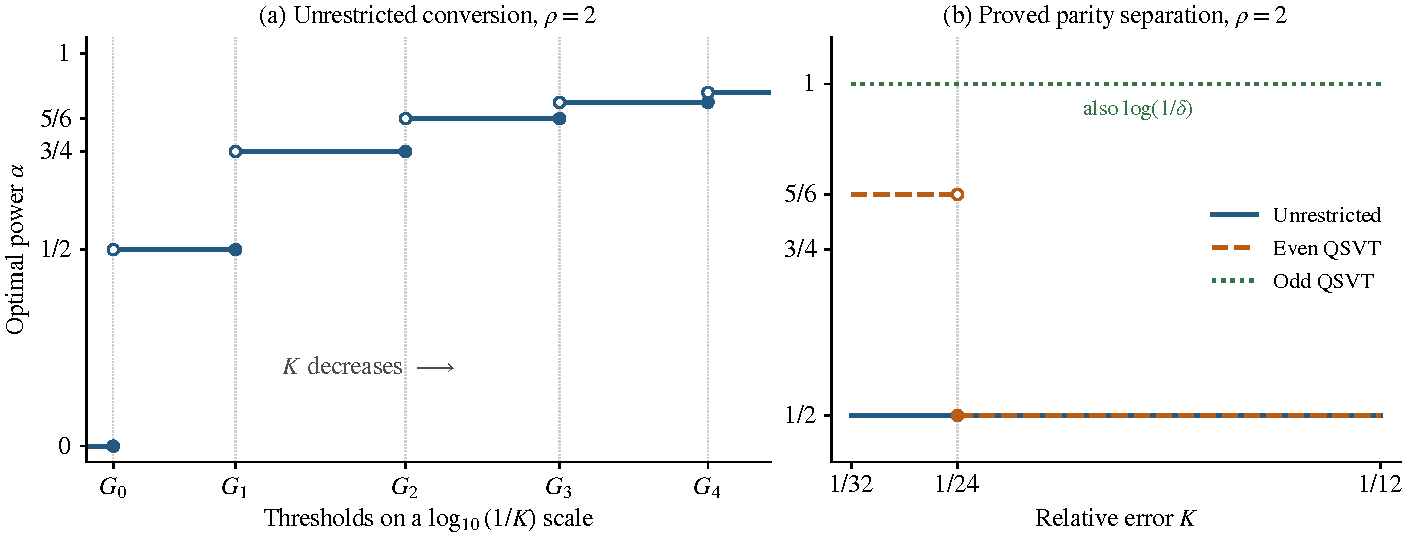
\includegraphics[width=\textwidth]{figures/query-overview.pdf}
\caption{Optimal query powers for fixed relative accuracy, with $\rho=2$. Left: the unrestricted exponent $\alpha$ in $Q=\delta^{-\alpha+o(1)}$ as $K$ decreases. At a threshold, a filled marker selects the cheaper tier; an open marker excludes the more expensive one. The coarse exponent zero includes a logarithmic cost for $c<1$. Right: the proved parity comparison on $1/32\leq K\leq1/12$. Because $F_1=F_2=1/24$, the even exponent jumps from $1/2$ to $5/6$; the odd class also has a logarithmic factor. The plot does not determine $F_3$. Threshold locations on the left are numerical evaluations of the exact formula in Theorem~\ref{thm:thresholds}; all complexity statements are proved.}\label{fig:overview}
\end{figure}

\subsection{Related work and contributions}
Quantum signal processing (QSP) and QSVT provide the tools we use to implement bounded polynomials. Gily\'en, Su, Low, and Wiebe \cite{gilyen2019} establish general singular value transformations, bounded approximations of the sign function, uniform amplification, and lower bounds for eigenvalue transformations from pairs of inputs. Low and Chuang \cite{low2017} develop uniform spectral amplification and track its normalization. Motlagh and Wiebe's GQSP \cite{motlagh2024} removes the usual definite-parity restriction by synthesizing bounded polynomials on the unit circle. We use these results, including a reduction to Laurent polynomials that works for arbitrary completions of the input block encoding; neither removing the parity restriction nor the generic amplification upper bound is our contribution. We count oracle queries and allow exact oracle-independent gates. Classical computation of phases and finite-precision circuit synthesis are separate questions; Haah \cite{haah2019} gives a rigorous algorithm for computing such phase decompositions and analyzes its cost.

The relation between analog quantum queries and trigonometric polynomials is known. Bessen \cite{bessen2004} uses it to compare real-valued query models, and Laneve \cite{laneve2026} characterizes QSP through state conversion and adversary feasibility. Our reduction to a scalar oracle is an instance of this polynomial method. What we add is the combination of two constraints: the circuit is unitary for every value of the scalar oracle, but it must be correct only on an interval that shrinks with $\delta$. After the rescaling $x=\delta y$ and division by $\delta$, any limit of the low-degree Taylor polynomials of $1-\operatorname{Re}q$, where $q$ is the output amplitude, must be nonnegative on all of $\R$. This leads to the extremal problem that defines $G_r$ and gives lower bounds for all coherent circuits, not only single QSP sequences. The pairwise square-root lower bound alone does not give the higher tiers.

In constrained polynomial approximation, Taylor \cite{taylor1968} studies restricted ranges, Lewis \cite{lewis1973} treats convex constraints, and Campos-Pinto, Charles, and Despr\'es \cite{campos2019} develop algorithms for positive polynomial approximation. Fawzi, Saunderson, and Parrilo \cite[Sections 3.1--3.2 and Appendix A, Lemma 1]{fawzi2017} study globally nonnegative interpolation of affine targets at finite nodes and use supporting tangents of Chebyshev polynomials; our threshold problem instead minimizes the uniform error on $[1,\rho]$. Its solution uses the classical Chebyshev inequality outside an interval, as stated for example by Bos, Ma'u, and Waldron \cite[Proposition 2.1]{bos2020}; our quantitative lower bounds also use the classical Fej\'er--Riesz factorization. The odd upper bound uses known sign approximations from QSVT, with antecedents in approximation theory by Eremenko and Yuditskii \cite{eremenko2007,eremenko2011}; the resulting degree of order (inverse gap) times $\log(1/\text{error})$ is not new. We use it for matching odd-polynomial bounds, with an elementary lower bound that uses correctness only on the low band.

Sarkar and Yoder \cite{sarkar2023} prove qualitative density results for QSP-related polynomial families with range constraints inside and outside the approximation interval, under necessary matching conditions at the endpoints, and study approximation of step functions; we ask for quantitative degree thresholds and coherent query costs as the correctness interval shrinks.

A particularly close recent work is that of Dong, Larsen, Lin, and Sarkar \cite{dong2026}. They formulate the design of QSP polynomials with prescribed parity as minimax fitting on a subset subject to a global bound on the modulus, study Remez methods with active constraints, and introduce a nonlinear Fourier retraction that restores feasibility without increasing the degree. Their work shows why bounds checked at sampled points are not enough, especially near the boundary of the feasible set. We address an analytic asymptotic question for one target and one spectral promise: exact limiting thresholds, optimal query powers over all circuits, and constructions that attain the threshold error. We prove on continuous domains that these constructions are bounded by one on $[-1,1]$ and that their error does not exceed the threshold, even at the points where the limiting error equals it; numerical plots are only illustrations. We do not propose a general minimax solver or a phase-synthesis algorithm.

In their Section 4.3, Orsucci and Dunjko \cite{orsucci2021}, our most direct motivation, also invoke QSVT lower bounds against generic amplification and give constructions from sparse matrix values for diagonally dominant matrices and for local sums of positive semidefinite terms; our analysis of plain block encodings does not resolve their question of a general construction from sparse matrix values. Their factor-based algorithms also explain square-root improvements in the condition number and the associated requirement on support overlap. Factor and sum-of-squares access are also central to the spectral amplification of King et al.\ \cite{king2026}. Somma and de Wolf \cite{somma2026} prove joint lower bounds for guided ground-state energy estimation and state preparation, including sum-of-squares access, under assumptions on guide overlap and dimension. Their tasks and hypotheses differ from ours, and we do not claim that their bounds apply here. Our state upper bounds for the LP use standard amplitude estimation \cite{brassard2002}.

Our contributions are: explicit formulas for the thresholds $G_r$ of the globally nonnegative approximation problem, and the complete fixed-accuracy query staircase for converting $H$ to $I-H$; the equality $F_1=F_2$ and the resulting sharp parity separation; lower bounds for interval spectra, uniform in the accuracy, that match the amplification cost when $K\leq\delta^\beta$, and a bound on the remaining gap at intermediate accuracy; and an explicit exactly central LP with fully specified oracles and matching bounds under access to the normal matrix and to its factor. To our knowledge, this combination of exact thresholds, constructions that attain the threshold error, and optimal query exponents for converting $H$ to $I-H$ has not appeared in the cited literature. This claim concerns the stated problem and theorems, not the underlying techniques of synthesis, approximation, or factor access.

\subsection{Organization}
Section~\ref{sec:model} connects block encodings to bounded polynomials and represents circuits with a scalar oracle by trigonometric polynomials. Section~\ref{sec:exact} contrasts finite known spectra with interval promises. In Section~\ref{sec:fixed}, global unitarity forces a nonnegative Taylor limit, Chebyshev growth outside an interval gives the thresholds, and a polynomial gate pinned to one where the approximation error equals $+G_r$ turns the extremal polynomial of the threshold problem into a converter bounded by one with error at most the threshold. Section~\ref{sec:joint} replaces fixed-order compactness by uniform Taylor estimates and an independent Fej\'er--Riesz argument, and controls the pinned construction when the order grows. Section~\ref{sec:lp} treats the LP. Section~\ref{sec:conclusion} lists open questions, and Appendix~\ref{app:reproduce} describes how to reproduce Figure~\ref{fig:overview} and build the source.

\section{Access model and polynomial implementation}\label{sec:model}
An exact block encoding of a Hermitian contraction $H$ is a unitary $U$ and a known isometry $J\colon v\mapsto |0^a\rangle\otimes v$, with $J^*UJ=H$. A unit-normalized $\eta$-approximate block encoding of $A$ is a unitary $V$ and a known isometry $J_{\mathrm{out}}$ such that
\[
 \norm{J_{\mathrm{out}}^*VJ_{\mathrm{out}}-A}\leq\eta.
\]
An exact block encoding of $A$ with normalization $\nu>0$ instead satisfies $J_{\mathrm{out}}^*VJ_{\mathrm{out}}=A/\nu$; unit normalization means $\nu=1$.
All operator norms are spectral norms. A converter is a circuit whose gates may depend on the stated spectral promise and accuracy, but not on the unknown matrix or on the completion of its oracle. It must work for every unitary $U$ with the prescribed compressed block. One controlled call to $U$ or $U^*$ costs one query. Ancillas, inverse calls, and coherently controlled choices of queries are allowed. The output is a reusable unitary; it is not conditioned on a favorable measurement outcome. If the worst-case query count is bounded, intermediate measurements can be deferred and their classical controls made coherent, so the lower bounds below cover this form of adaptivity. We do not consider algorithms with unbounded stopping times and bounded expected cost.

The main spectral promise is
\begin{equation}\label{eq:bands}
 0<\delta,\qquad \rho>1,\qquad 0<c\leq1,\qquad
 \rho\delta<c,\qquad
 \spec(H)\subseteq[\delta,\rho\delta]\cup[c,1].
\end{equation}
Let $Q(\delta,\eta;\rho,c)$ be the minimum worst-case query count for unit-normalized conversion to $I-H$ under this promise, uniformly in the matrix dimension. Constants in asymptotic notation may depend on the fixed parameters shown as subscripts. In the fixed-relative-accuracy results, $\rho,c,K$ are fixed and $\eta=K\delta$ as $\delta\downarrow0$.

\begin{lemma}[Bounded polynomial implementation]\label{lem:implementation}
If $p\in\R[x]$ has degree $d$ and $|p(x)|\leq1$ on $[-1,1]$, then $p(H)$ has an exact unit-normalized block encoding using $O(d)$ controlled queries to any exact block encoding of the Hermitian contraction $H$. If $p$ has definite parity, $d$ queries suffice in the real-polynomial QSVT convention.
\end{lemma}
\begin{proof}
The definite-parity statement is the real-polynomial singular value transformation theorem of Gily\'en et al.\ \cite[Corollary 18, extended version]{gilyen2019}. It extracts the real part by coherently averaging the phase sequences with opposite signs; this uses an extra qubit and loses no normalization. For any Hermitian $H$, the even transform gives $p(|H|)=p(H)$, while the odd transform includes the left/right singular-vector signs and gives $\operatorname{sign}(H)p(|H|)=p(H)$. On the zero eigenspace the odd case follows from $p(0)=0$.

For completeness, we give the reduction for polynomials without definite parity; it makes no assumption on the unknown completion. Define the Hermitian unitary
\[
 \widetilde U=|0\rangle\langle1|\otimes U+
 |1\rangle\langle0|\otimes U^*,\qquad
 \widetilde J=|+\rangle\otimes J.
\]
Its compression is $H$, and it costs a constant number of controlled oracle calls. Set $\Pi=\widetilde J\widetilde J^*$ and $V=(2\Pi-I)\widetilde U$. For each eigenvector $v$ of $H$ with eigenvalue $x\in(-1,1)$, the span of $\widetilde Jv$ and $(\widetilde U\widetilde Jv-x\widetilde Jv)/\sqrt{1-x^2}$ is invariant, and $V$ has matrix
\[
 \begin{pmatrix}x&\sqrt{1-x^2}\\-\sqrt{1-x^2}&x\end{pmatrix}.
\]
Thus $(V+V^*)/2=xI$ on this subspace; the endpoint eigenspaces follow directly. The ordinary polynomial
\[
 R(z)=z^d p\bigl((z+z^{-1})/2\bigr)
\]
has degree at most $2d$ and modulus at most one on the unit circle. Generalized quantum signal processing (GQSP) \cite{motlagh2024}, via a Fej\'er--Riesz completion, implements $R(V)$ with at most $2d$ controlled walk queries. Multiplication by $V^{-d}$ uses another $d$ queries and gives $p((V+V^*)/2)$. Compression by $\widetilde J$ gives $p(H)$. The construction is coherent and unit-normalized throughout.
\end{proof}

\begin{lemma}[Scalar representation and derivative bounds]\label{lem:scalar}
For the scalar oracle
\begin{equation}\label{eq:scalar-oracle}
 U(t)=\begin{pmatrix}\sin t&\cos t\\\cos t&-\sin t\end{pmatrix},
\end{equation}
each matrix element $q(t)$ of a $T$-query converter is a trigonometric polynomial of degree at most $T$ and satisfies $|q(t)|\leq1$ for every real $t$. The function $g(x)=1-\operatorname{Re}q(\arcsin x)$ obeys $0\leq g\leq2$ on $[-1,1]$ and, for each fixed integer $j\geq1$,
\begin{equation}\label{eq:derivative-bound}
 \sup_{|x|\leq1/2}|g^{(j)}(x)|\leq C_j(T+1)^j.
\end{equation}
\end{lemma}
\begin{proof}
The entries of each query, including a controlled query whose inactive block is the identity, have trigonometric degree at most one. Each query therefore increases the degree of the entries by at most one. Gates that do not depend on the oracle, and ancillas, do not affect this induction. Unitarity bounds each output entry for all $t$, whether or not $\sin t$ satisfies the spectral promise. Trigonometric Bernstein inequalities bound the $j$th derivative in $t$ by $2T^j$ for $1-\operatorname{Re}q(t)$. Repeated differentiation of $t=\arcsin x$, whose derivatives of every fixed order are bounded on $[-1/2,1/2]$, proves \eqref{eq:derivative-bound}.
\end{proof}

\section{Exact conversion: known finite spectra versus intervals}\label{sec:exact}
\begin{proposition}[Two-query conversion]\label{prop:two-point}
Let $0<a<b\leq1$ be known, with $(1-a)(1-b)\leq a+b$. The polynomial
\[
 p_{a,b}(x)=1-\frac{ab+x^2}{a+b}
\]
is bounded in absolute value by one on $[-1,1]$. Two QSVT queries implement it, and
\begin{equation}\label{eq:quadratic-error}
 p_{a,b}(H)-(I-H)=-\frac{(H-aI)(H-bI)}{a+b}.
\end{equation}
Consequently the conversion is exact if $\spec(H)\subseteq\{a,b\}$; for any other spectrum its error is exactly
$\max_{x\in\spec(H)}|(x-a)(x-b)|/(a+b)$.
\end{proposition}
\begin{proof}
The polynomial decreases as $x^2$ increases. Its maximum is $1-ab/(a+b)<1$, and its minimum is $-(1-a)(1-b)/(a+b)\geq-1$. The remaining assertions follow from Lemma~\ref{lem:implementation} and factorization.
\end{proof}
In particular, $b\geq1/2$ suffices for the hypothesis, and $b=1$ gives $p_{a,1}(x)=(1-x^2)/(1+a)$. Thus a large condition number alone does not make unit-normalized conversion to $I-H$ expensive. This result concerns the conversion of an operator; it does not remove the normalization and overlap costs of a linear-system output state.

\begin{proposition}[An interval cannot be converted exactly]\label{prop:no-exact}
No finite-query converter produces an exact encoding of $I-H$ with normalization $0<\nu<2$ for every scalar $H=x$ in any nonempty open subinterval of $(0,1)$.
\end{proposition}
\begin{proof}
By Lemma~\ref{lem:scalar}, the designated output entry $q(t)$ of such a converter is a trigonometric polynomial. By analyticity, equality with $(1-\sin t)/\nu$ on an open interval implies equality for every real $t$. At $t=-\pi/2$ this would give $q(t)=2/\nu>1$, contradicting unitarity.
\end{proof}

\begin{proposition}[Pairwise lower bound and normalization near one]\label{prop:pairwise}
Suppose $0<\delta\leq1/4$ and a converter works at both $H=\delta$ and $H=2\delta$ with error at most $\delta/16$. It uses at least
\[
 \frac{\sqrt3}{2}\left(\sqrt{\frac{93}{32}}-\sqrt{\frac{17}{8}}\right)\delta^{-1/2}
\]
queries. Moreover, the differentiated hybrid argument gives the following formal bound: if $\nu>1-\delta$ and an exact converter with normalization $\nu$ that uses $T$ queries works on a neighborhood of $x=\delta$, then
\begin{equation}\label{eq:normalization-slack}
 T\geq\frac{(1-\delta)\sqrt{1-\delta^2}}
 {\nu\sqrt{\nu^2-(1-\delta)^2}}.
\end{equation}
\end{proposition}
\begin{proof}
Use the canonical oracle $U(\arcsin x)$. Its derivative in $x$ has norm $1/\sqrt{1-x^2}$, so the hybrid argument gives
\[
 \norm{V_{2\delta}-V_\delta}\leq\frac{2T\delta}{\sqrt3}.
\]
Apply each output unitary to its designated input basis vector. If the designated output amplitude is $z$, the component orthogonal to the designated output has norm $\sqrt{1-|z|^2}$. At $x=\delta$ this norm is at most $\sqrt{17\delta/8}$, since $|z|\geq1-17\delta/16$. At $x=2\delta$ it is at least $\sqrt{93\delta/32}$: indeed $|z|\leq1-31\delta/16$, and $1-(1-s)^2\geq3s/2$ for $s=31\delta/16\leq1/2$. The difference between these norms bounds the distance between the output vectors from below, proving the first claim.

For the second claim, the exact designated amplitude is $f(x)=(1-x)/\nu$. The norm of the orthogonal component has derivative $(1-x)/(\nu\sqrt{\nu^2-(1-x)^2})$. Compare neighboring inputs, apply the hybrid argument with oracle derivative $1/\sqrt{1-x^2}$, divide by their separation, and take the limit.
\end{proof}
The pairwise method is a special case of the lower-bound method for eigenvalue transformations in \cite[Theorem 73, extended version]{gilyen2019}. The differentiated inequality \eqref{eq:normalization-slack} is only formal and gives no lower bound: Proposition~\ref{prop:no-exact} rules out its hypothesis for every $\nu<2$, and for $\nu\geq2$ its right side is less than one. It only shows how the local obstruction grows as $\nu$ decreases to $1-\delta$. At normalization two, a direct coherent linear combination implements $(I-H)/2$ with a constant number of queries. The rest of the paper studies how the cost at normalization one depends on the accuracy.

\section{The complete fixed-relative-accuracy staircase}\label{sec:fixed}
All approximation-order indices, including $r$ and $j$, are nonnegative integers. For $r\geq0$ define
\begin{equation}\label{eq:G-definition}
 G_r(\rho)=\inf\left\{\max_{1\leq y\leq\rho}|P(y)-y|:
 P\in\R[y],\ \deg P\leq2r,\ P\geq0\text{ on }\R\right\}.
\end{equation}
The constraint on the entire real line is essential: the approximation error is measured only on $[1,\rho]$.

\begin{theorem}[Optimal fixed-accuracy queries]\label{thm:staircase}
Fix $\rho>1$, $0<c\leq1$, and $K>0$, and put
$\ell=\min\{j\geq0:G_j(\rho)\leq K\}$.
Then $\ell$ is finite and, as $\delta\downarrow0$,
\begin{equation}\label{eq:staircase}
 Q(\delta,K\delta;\rho,c)=
 \begin{cases}
 \Theta_{\rho,c,K}(\log(1/\delta)),&\ell=0,\quad c<1,\\
 \Theta_{\rho,K}(1),&\ell=0,\quad c=1,\\
 \Theta_{\ell,\rho,c,K}(\delta^{-1+1/(2\ell)}),&\ell\geq1.
 \end{cases}
\end{equation}
Every threshold equality $K=G_\ell$ belongs to the cheaper tier displayed in this formula.
\end{theorem}
The distinction at $c=1$ has a simple cause: $[c,1]$ is then a single known spectral point. A high interval of positive length supplies an additional logarithmic obstruction, whereas one known point can be handled by interpolation.

\subsection{The globally nonnegative approximation problem}
Write
\[
 m_\rho=\frac{\rho+1}{2},\qquad h_\rho=\frac{\rho-1}{2},\qquad
 z_0=\frac{m_\rho}{h_\rho},
\]
and let $T_n$ denote the Chebyshev polynomial, $T_n(\cos\theta)=\cos(n\theta)$.
\begin{theorem}[Exact thresholds]\label{thm:thresholds}
We have $G_0=h_\rho$. For $r\geq1$,
\begin{align}
 G_r&=h_\rho\max_{z\geq z_0}\frac{z-z_0}{T_{2r}(z)},\label{eq:G-formula}\\
 P_r^*(y)&=y+G_r T_{2r}\bigl((y-m_\rho)/h_\rho\bigr)\label{eq:extremizer}
\end{align}
are respectively the optimal error and an admissible minimizer. The positive numbers $G_r$ strictly decrease to zero. If $z_*$ is the maximizer in \eqref{eq:G-formula}, it is unique and
\begin{equation}\label{eq:G-stationary}
 z_*-z_0=T_{2r}(z_*)/T_{2r}'(z_*),\qquad
 G_r=h_\rho/T_{2r}'(z_*).
\end{equation}
\end{theorem}
\begin{proof}
The constant case is ordinary interval minimax approximation. For $n=2r\geq2$, the exterior Chebyshev inequality says that a degree-at-most-$n$ polynomial $A$ bounded by one on $[-1,1]$ satisfies $|A(z)|\leq T_n(|z|)$ for $|z|>1$. One elementary proof compares $A$ with $T_n$ at its $n+1$ successive extrema: if the exterior inequality failed, subtracting a suitable multiple of $T_n$ would give $n$ interior sign changes and an exterior zero, contradicting the degree. Apply this inequality to $P(y)-y$. At $y=-h_\rho(z-z_0)\leq0$, nonnegativity gives $P(y)-y\geq h_\rho(z-z_0)$, proving the lower bound in \eqref{eq:G-formula}.

To prove admissibility of \eqref{eq:extremizer}, set $e=G_r/h_\rho$ and $x=(y-m_\rho)/h_\rho$. We must show $x+z_0+eT_n(x)\geq0$ for every real $x$. For $x\leq-z_0$ this is precisely the maximizing inequality defining $e$. For $-z_0\leq x\leq-1$ and for $x\geq1$, both terms are nonnegative. On $[-1,1]$, only negative lobes of $T_n$ require attention. They satisfy $x\geq-\cos(\pi/(2n))$, so
\[
 x+z_0>1-\cos(\pi/(2n))\geq n^{-2}.
\]
The last bound follows from $\sin u\geq2\sqrt2 u/\pi$ on $[0,\pi/4]$. Since $T_n$ is strictly convex on $[1,\infty)$ and $T_n'(1)=n^2$,
$T_n(z)\geq1+n^2(z-1)$, whence $e<n^{-2}$. Since $T_n(x)\geq-1$, positivity follows. The approximation error is exactly $G_r$ by Chebyshev alternation.

The maximum in \eqref{eq:G-formula} is positive, attained away from $z_0$ and infinity. The function $z-T_n(z)/T_n'(z)$ increases strictly on $(1,\infty)$, with derivative $T_nT_n''/(T_n')^2>0$, and tends to infinity. This proves uniqueness and \eqref{eq:G-stationary}. For successive positive indices, evaluate the ratio for $T_{2r+2}$ at its maximizer and use $T_{2r+2}(z)>T_{2r}(z)$ for $z>1$. Also $G_1<G_0$: the explicit formula below proves this directly. Finally, polynomial approximations to $\sqrt y$ on $[1,\rho]$, squared, are globally nonnegative and converge uniformly to $y$. Thus $G_r\to0$.
\end{proof}
The admissibility has a geometric antecedent: by \eqref{eq:G-stationary}, in the coordinate $z=(m_\rho-y)/h_\rho$, the extremizer is $G_r$ times the difference between $T_{2r}(z)$ and its tangent at $z_*$. Its nonnegativity also follows from the supporting-tangent inequality of Fawzi, Saunderson, and Parrilo \cite[Appendix A, Lemma 1]{fawzi2017}; the proof above is self-contained.

For the first threshold the formula simplifies to
\begin{equation}\label{eq:G1}
 G_1=\frac{\rho+1-\sqrt{(\rho^2+6\rho+1)/2}}4,
 \qquad P_1^*(y)=\frac{(y+s)^2}{2(m_\rho+s)},\quad
 s=\sqrt{m_\rho^2-h_\rho^2/2}.
\end{equation}
These expressions follow either by solving \eqref{eq:G-stationary} for $T_2(z)=2z^2-1$ or by expanding \eqref{eq:extremizer}.

\begin{proposition}[Threshold asymptotics]\label{prop:threshold-asymptotics}
Let $R_0=(\sqrt\rho+1)/(\sqrt\rho-1)$ and $a=\log R_0$. As $r\to\infty$,
\begin{equation}\label{eq:G-asymptotic}
 G_r=\frac{\sqrt\rho}{\mathrm e\,r}R_0^{-2r}
 (1+O_\rho(r^{-1})).
\end{equation}
Consequently, as $K\downarrow0$, with $L=\log(1/K)$,
\[
 \ell(K)=\frac{L-\log L+\log(2\sqrt\rho\,a/\mathrm e)}{2a}+O_\rho(1),
 \qquad
 1-\frac1{2\ell(K)}
 =1-\frac{a}{L-\log L+O_\rho(1)}.
\]
The $O(1)$ term in the first expression includes integer rounding.
\end{proposition}
\begin{proof}
Put $n=2r$, $z=\cosh t$, and note $z_0=\cosh a$. The stationary equation is
\[
 n(\cosh t-\cosh a)\tanh(nt)=\sinh t.
\]
Its solution has $t=a+O_\rho(n^{-1})$: indeed the increasing left-to-right ratio $n(\cosh t-\cosh a)/\sinh t$ crosses one within such a neighborhood, and $\tanh(nt)=1+O_\rho(e^{-2na})$. Expanding with $t=a+s/n$ now gives $s=1+O_\rho(n^{-1})$. Substitution into \eqref{eq:G-formula}, using $h_\rho\sinh a=\sqrt\rho$, gives \eqref{eq:G-asymptotic}. Taking logarithms and inverting $L=2ar+\log r-\log(\sqrt\rho/\mathrm e)+O_\rho(1/r)$ gives the last claims, with bounded rounding uncertainty.
\end{proof}

\subsection{An all-circuit lower bound}
\begin{theorem}[Nonnegative Taylor limit]\label{thm:hierarchy}
Fix $r\geq0$ and $K<G_r(\rho)$. Any coherent converter accurate to $K\delta$ on $[\delta,\rho\delta]$ uses
\[
 T=\Omega_{r,\rho,K}(\delta^{-(2r+1)/(2r+2)})
\]
queries. No upper spectral interval is needed for this bound.
\end{theorem}
\begin{proof}
Use Lemma~\ref{lem:scalar} and put $g_\delta(x)=1-\operatorname{Re}q_\delta(\arcsin x)$. Correctness implies
\[
 |g_\delta(\delta y)/\delta-y|\leq K\qquad(1\leq y\leq\rho).
\]
Taylor expansion through order $2r+1$, followed by rescaling, gives a polynomial $A_\delta$ of degree at most $2r+1$ such that, on each fixed compact set of real $y$,
\[
 g_\delta(\delta y)/\delta=A_\delta(y)
 +O_{r,y}((T+1)^{2r+2}\delta^{2r+1}).
\]
If the claimed bound failed, there would be a sequence $\delta\downarrow0$ with $T\delta^{(2r+1)/(2r+2)}\to0$, so the remainder would vanish uniformly on each fixed compact set. Values at $2r+2$ fixed distinct points of $(1,\rho)$ then bound all coefficients of $A_\delta$ by invertibility of the Vandermonde matrix. Pass to a coefficientwise convergent subsequence, with limit $A$. For each fixed real $y$, global nonnegativity of $g_\delta$ gives $A(y)\geq0$. A nonzero nonnegative polynomial has even degree; thus $\deg A\leq2r$. It approximates $y$ within $K$ on $[1,\rho]$, contradicting the definition of $G_r$.
\end{proof}
If $\eta(\delta)/\delta\to0$, this immediately yields $T=\Omega_{\rho,\varepsilon}(\delta^{-1+\varepsilon})$ for every fixed $\varepsilon>0$ (with the onset depending on the accuracy function). This is stronger than the pairwise square-root obstruction. It uses contractivity outside the correctness interval, through the globally nonnegative Taylor limit.

\subsection{Bounded constructions, including exact threshold errors}
We first record a positive approximant for the fixed upper interval. Define $d_j$ by
\[
 \frac{1-\sqrt{1-z}}{1-z}=\sum_{j\geq1}d_jz^j,\qquad
 S_N(u)=u\sum_{j=1}^N d_j(1-u)^j.
\]
The coefficients $d_j$ are partial sums of the positive Taylor coefficients of $1-\sqrt{1-z}$, so $0<d_j\leq1$. For $0\leq u\leq1$,
\begin{equation}\label{eq:SN}
 0\leq S_N(u)\leq1-\sqrt u,\quad
 0\leq1-\sqrt u-S_N(u)\leq(1-u)^{N+1},\quad S_N(u)\leq Nu.
\end{equation}
The tail estimate follows by comparison with the geometric series; the endpoints follow by continuity. For $c<1$, $N=O_c(\log(1/\delta))$ makes the high-band tail any prescribed constant multiple of $\delta$. For $c=1$, $N=1$ suffices because $S_N(1)=0$.

\begin{lemma}[A pinned gate]\label{lem:pinned}
Fix $r\geq1$ and a nonempty finite set $A\subseteq[1,\rho]$. Put $\alpha=1-1/(2r)$ and choose an odd integer $m\asymp M\delta^{-\alpha}$, where $M>0$ is fixed. There is an even polynomial $W$ of degree $O_{r,|A|}(m)$ with $0\leq W\leq1$ on $[-1,1]$, $W(\delta y)=1$ for $y\in A$, and
\begin{align}
 1-W(\delta y)&\leq C(m\delta)^{2r+2}\dist(y,A)^{2r+2},
 &&1\leq y\leq\rho,\label{eq:pinned-low}\\
 W(x)&\leq C(m|x|)^{-2r-4},&& C_0\delta\leq|x|\leq1.\label{eq:pinned-tail}
\end{align}
Constants may depend on $r,\rho,A$, but not on $\delta,m$; $C_0$ is chosen sufficiently large depending on $\rho$.
\end{lemma}
\begin{proof}
For $\theta_j=\arcsin(\delta y_j)$, $y_j\in A$, define
\[
 D_{m,a}(\theta)=\frac{\sin(m(\theta-a))}{m\sin(\theta-a)},\quad
 W(\sin\theta)=1-
 \prod_{y_j\in A}\prod_{\sigma=\pm1}
 \left(1-D_{m,\sigma\theta_j}(\theta)^{2r+4}\right)^{r+1}.
\]
Removable singularities are filled by continuity. The elementary inequality $|\sin(mu)|\leq m|\sin u|$ gives $|D_{m,a}|\leq1$. For odd $m$, $D_{m,a}$ is a real trigonometric polynomial with even frequencies and degree $m-1$. Pairing $a$ with $-a$ makes the product even in $\theta$ and $\pi$-periodic. It is therefore a polynomial in $\cos2\theta=1-2x^2$, of degree $O_{r,|A|}(m)$ in $x$. The range and pinning properties are immediate.

Near a pin, $1-D_{m,a}(\theta)^{2r+4}\leq C_rm^2(\theta-a)^2$. Select the nearest positive pin in the product defining $1-W$ and bound all other factors by one. Since $|\arcsin(\delta y)-\arcsin(\delta y_j)|\leq2\delta|y-y_j|$ for small $\delta$, this proves \eqref{eq:pinned-low}. Finally, if $C_0\delta\leq|x|\leq1$, then $|\sin(\arcsin x\pm\theta_j)|\geq|x|/2$. Hence $|D_{m,\pm\theta_j}|\leq2/(m|x|)$. Applying $1-\prod_i(1-a_i)^{r+1}\leq(r+1)\sum_i a_i$ proves \eqref{eq:pinned-tail}.
\end{proof}

\begin{proposition}[Upper bound at every positive threshold]\label{prop:threshold-upper}
For each fixed $r\geq1$ there is a polynomial $q_\delta$ bounded by one on $[-1,1]$ with error at most $G_r\delta$ on \eqref{eq:bands} and degree $O_{r,\rho,c}(\delta^{-1+1/(2r)})$.
\end{proposition}
\begin{proof}
Take $P=P_r^*$ and $e(y)=P(y)-y$. The positive-contact set
$A=\{y\in[1,\rho]:e(y)=G_r\}$ is finite and nonempty, by \eqref{eq:extremizer}. Use Lemma~\ref{lem:pinned} for this set and define
\begin{equation}\label{eq:blend}
 q_\delta(x)=W(x)[1-\delta P(x/\delta)]+(1-W(x))S_N(x^2).
\end{equation}
We verify contractivity before its approximation property. Write $q_\delta=B-\delta P(x/\delta)W$ with $B=W+(1-W)S_N(x^2)\in[0,1]$. Thus $q_\delta\leq1$. Since $P(y)\leq C(1+|y|^{2r})$ and $P\geq0$, splitting at $|x|=C_0\delta$ and $|x|=1/m$ gives
\begin{equation}\label{eq:global-loss}
 0\leq\delta P(x/\delta)W(x)
 \leq C\delta+C\delta^{1-2r}m^{-2r}
 \leq C\delta+C'M^{-2r}.
\end{equation}
Indeed $C_0\delta<1/m$ for small $\delta$; on the middle region use $W\leq1$, and on the outer region use \eqref{eq:pinned-tail}. Choose $M$ large enough and then $\delta$ small enough to make \eqref{eq:global-loss} at most one. It follows that $q_\delta\geq-1$.

For the lower interval, the polynomial $G_r-e(y)$ is nonnegative on $[1,\rho]$ and has zeros there exactly at $A$, with multiplicities at most $2r$. Compactness and factorization therefore give a constant $b>0$ such that
\[
 G_r-e(y)\geq b\dist(y,A)^{2r}\quad(1\leq y\leq\rho).
\]
Since $(m\delta)^{2r+2}=O(\delta^{1+1/r})$, \eqref{eq:pinned-low} and $W=1-o(1)$ on this interval imply, for small $\delta$,
\begin{equation}\label{eq:pinned-slack}
 1-W(\delta y)\leq\tfrac12 W(\delta y)\delta[G_r-e(y)].
\end{equation}
This estimate includes the contacts themselves, where both sides vanish. Put $d(x)=1-x-S_N(x^2)\in[0,1]$ for $0\leq x\leq1$. On $x=\delta y$,
\[
 (1-x)-q_\delta(x)=W\delta e(y)+(1-W)d(x).
\]
Its lower bound is $-G_r\delta$ because $e\geq-G_r$ and $d\geq0$. Its upper bound follows from \eqref{eq:pinned-slack}:
\[
 G_r\delta-[(1-x)-q_\delta(x)]
 =W\delta(G_r-e)+(1-W)(G_r\delta-d)\geq0.
\]
Thus the error is at most exactly $G_r\delta$, without an asymptotic error overshoot.

On $[c,1]$, the tail in \eqref{eq:SN} can be made at most $G_r\delta/3$. Also $W=O(m^{-2r-4})=o(\delta)$, and
\[
 \delta P(x/\delta)W=O(\delta^{1-2r}m^{-2r-4})
 =O(\delta^{4-2/r})=o(\delta).
\]
These two terms can each be made at most $G_r\delta/3$ by decreasing $\delta$. Finally, \eqref{eq:blend} has degree $O_{r,\rho}(m+N)$, proving the claim.
\end{proof}
The pinned construction handles strict bands as well, by using the smallest $r$ with $G_r\leq K$. Pinning is necessary in this proof to control the sign of the error at the exact minimax contacts; a gate with merely $o(\delta)$ leakage would only establish errors $(G_r+o(1))\delta$.

\subsection{The coarse tier and completion of the staircase proof}
\begin{proposition}[Coarse conversion]\label{prop:coarse}
For $K\geq G_0=(\rho-1)/2$, the first two lines of \eqref{eq:staircase} hold.
\end{proposition}
\begin{proof}
It suffices to construct error $G_0\delta$. Set $P=m_\rho$, so $e(y)=m_\rho-y$ and $G_0-e(y)=y-1$. First suppose $c<1$ and use
\[
 W(x)=[1-(x^2-\delta^2)^2]^L,\qquad
 L=\lceil C_c\log(1/\delta)\rceil.
\]
For small $\delta$, the base is in $[0,1]$ on $[-1,1]$. On the lower band,
\[
 1-W(\delta y)\leq L\delta^4(y^2-1)^2
 \leq C_\rho L\delta^4(y-1)^2.
\]
This is at most $\tfrac12W\delta(y-1)$ for sufficiently small $\delta$. On the high band, $W\leq(1-c^4/4)^L$ for $\delta$ sufficiently small. Choose the constant in $L$ so that this leakage is at most $G_0\delta/3$, and choose $N=O_c(\log(1/\delta))$ so the tail in \eqref{eq:SN} is at most $G_0\delta/3$. The blend \eqref{eq:blend} is a convex combination of $1-m_\rho\delta$ and $S_N(x^2)$, hence lies in $[0,1]$. The same signed-error argument as in Proposition~\ref{prop:threshold-upper} proves the exact low-band error. On the high band its error is at most the tail plus $W$, which is below $G_0\delta$. Its degree is $O(\log(1/\delta))$.

If $c=1$, instead take
\[
 W(x)=1-\left(\frac{x^2-\delta^2}{1-\delta^2}\right)^2,
 \qquad q_\delta(x)=(1-m_\rho\delta)W(x).
\]
For small $\delta$, $0\leq W\leq1$ on $[-1,1]$, $W(\delta)=1$, and $W(1)=0$. The low leakage is $O_\rho(\delta^4(y-1)^2)$ and the same signed-error argument applies with $S_N=0$. This degree-four polynomial is exact at the high point $1$. A zero-query circuit has the same scalar output at $x=\delta$ and $x=1$, whose targets differ by $1-\delta$, so cannot satisfy the error contract for small $\delta$. This gives $\Theta(1)$.

For the logarithmic lower bound when $c<1$, choose a closed interval $I$ of positive length $b$ strictly inside $(\arcsin c,\pi/2)$. Let $q(t)$ be the scalar output entry and $R(t)=q(t)-(1-\sin t)$. It has trigonometric degree $n\leq\max(T,1)$, is bounded by $K\delta$ on $I$, and satisfies $|R(-\pi/2)|\geq1$ by contractivity. Here is a direct form of the needed interpolation inequality. If $R$ has degree at most $n$, then $z^nR(t)$, $z=e^{it}$, is an ordinary polynomial of degree at most $2n$. Interpolate at $2n+1$ equally spaced angles in $I$. For node indices $i,j$, their distance on the unit circle is at least $b|i-j|/(\pi n)$, whereas its distance to any evaluation point on the unit circle is at most two. The sum of the absolute Lagrange weights is consequently at most
\[
 \left(\frac{2\pi n}{b}\right)^{2n}
 \sum_{j=0}^{2n}\frac1{j!(2n-j)!}
 =\frac{(4\pi n/b)^{2n}}{(2n)!}
 \leq(2\pi\mathrm e/b)^{2n}.
\]
Thus $1\leq K\delta(2\pi\mathrm e/b)^{2n}$, giving $T=\Omega_{c,K}(\log(1/\delta))$.
\end{proof}
\begin{proof}[Proof of Theorem~\ref{thm:staircase}]
Theorem~\ref{thm:thresholds} guarantees existence of $\ell$. For $\ell\geq1$, the lower bound is Theorem~\ref{thm:hierarchy} with $r=\ell-1$, since $K<G_{\ell-1}$. Proposition~\ref{prop:threshold-upper}, followed by Lemma~\ref{lem:implementation}, gives the matching upper bound because $G_\ell\leq K$. Proposition~\ref{prop:coarse} treats $\ell=0$.
\end{proof}

\subsection{Definite parity and a polynomial query separation}
Even polynomials satisfy additional lower bounds governed by the following approximation errors. Define
\[
 E_r(\rho)=\inf_{A\in\R[v],\,\deg A\leq r}
 \max_{1\leq y\leq\rho}|y-A(y^2)|.
\]
These unconstrained errors first give elementary lower-bound cutoffs. Retaining global nonnegativity below will give an optimal implicit even-parity staircase, including equality cases. Each $E_r$ is positive: otherwise finite-dimensional compactness would give an exact polynomial representation of $\sqrt v$ on $[1,\rho^2]$, which is impossible. In particular, the affine cutoff is
\begin{equation}\label{eq:E1}
 E_1=\frac{(\rho-1)^2}{8(\rho+1)},\qquad
 A_1(v)=a_\rho v+b_\rho,\quad
 a_\rho=\frac1{\rho+1},\quad
 b_\rho=\frac\rho{\rho+1}+E_1.
\end{equation}
To verify minimax optimality, the error $\sqrt v-A_1(v)$ equals $-E_1$ at $v=1,\rho^2$, and $E_1$ at $v=(\rho+1)^2/4$. An affine perturbation reducing all three absolute errors would need two sign changes, which is impossible.

\begin{proposition}[Parity obstructions]\label{prop:parity-lower}
Let $p$ be a real polynomial bounded by one on $[-1,1]$ that approximates $1-x$ within $K\delta$ on $[\delta,\rho\delta]$. If $p$ is even and $K<E_r(\rho)$, then
\[
 \deg p=\Omega_{r,\rho,K}(\delta^{-1+1/(2r+2)}).
\]
More explicitly, if $\deg p=2m$ and $K<E_1$, then
\begin{equation}\label{eq:even-explicit}
 m\geq\left(\frac{3(E_1-K)}{2\rho^4}\right)^{1/4}\delta^{-3/4}.
\end{equation}
If $p$ is odd, then
\[
 \deg p\geq\frac{[1-(1+K)\delta]\sqrt{1-\delta^2}}{\delta}.
\]
\end{proposition}
\begin{proof}
Taylor-expand an even degree-$d$ polynomial at zero through degree $2r$. On a fixed interior subinterval, Bernstein inequalities give $|p^{(j)}|\leq C_j(d+1)^j$ for each fixed $j$. The vanishing odd Taylor terms imply that $(1-p(\delta y))/\delta$ differs from a degree-$r$ polynomial in $y^2$ by at most $C_{r,\rho}(d+1)^{2r+2}\delta^{2r+1}$. Therefore
$E_r\leq K+C_{r,\rho}(d+1)^{2r+2}\delta^{2r+1}$, giving the first claim.
For the explicit constant, write $p(x)=A(x^2)$ with $\deg A=m$ and $\norm{A}_{[0,1]}\leq1$. The second Markov inequality on $[0,1]$ gives $\norm{A''}\leq4m^2(m^2-1)/3$. The first-order Taylor remainder at $u=\delta^2v$, divided by $\delta$, is at most $2m^4\rho^4\delta^3/3$. Comparing to the best affine error proves \eqref{eq:even-explicit}. Finally, odd parity gives $p(0)=0$, so the mean-value theorem and Bernstein's first-derivative inequality give
$(1-(1+K)\delta)/\delta\leq\sup_{[0,\delta]}|p'|\leq d/\sqrt{1-\delta^2}$.
\end{proof}

\begin{proposition}[Even square-root construction]\label{prop:even-upper}
For every fixed $\gamma>0$, there is an even polynomial bounded by one on $[-1,1]$ with error at most $(E_1+\gamma)\delta$ on \eqref{eq:bands} and degree $O_{\rho,c,\gamma}(\delta^{-1/2})$.
\end{proposition}
\begin{proof}
For an integer $m\geq2$ define the normalized endpoint Fej\'er kernel
\[
 F_m(u)=\frac{1-T_m(1-2u)}{2m^2u},\quad F_m(0)=1.
\]
This is a polynomial of degree $m-1$. If $u=\sin^2(\theta/2)$, then
$F_m(u)=\sin^2(m\theta/2)/(m^2\sin^2(\theta/2))$, so
$0\leq F_m\leq1$ on $[0,1]$ and $F_m(u)\leq1/(m^2u)$ for $0<u\leq1$.
Taylor expansion at zero gives
\[
 F_m(u)=1-\frac{m^2-1}{3}u+O(m^4u^2).
\]
The remainder is uniform when $m^2u=o(1)$; it also follows from the second Markov bound and $\norm{F_m}_{[0,1]}\leq1$.
Choose an integer $m$ nearest the positive solution of
$2(m^2-1)\delta/3=a_\rho$ and set $W_m=F_m^2$. Integer rounding gives, uniformly on $1\leq v\leq\rho^2$,
\[
 1-W_m(\delta^2v)=a_\rho\delta v+O_\rho(\delta^{3/2}).
\]
Using \eqref{eq:SN} with a high-band tail $O(\delta^2)$, define
\[
 P_\delta(u)=(1-b_\rho\delta)W_m(u)+(1-W_m(u))S_N(u),
 \qquad p_\delta(x)=P_\delta(x^2).
\]
This is a convex combination of numbers in $[0,1]$. On the low band, $S_N(\delta^2v)=O(N\delta^2)$ and hence
\[
 1-P_\delta(\delta^2v)=\delta(b_\rho+a_\rho v)
 +O_{\rho,c}(\delta^{3/2}+\delta^2\log(1/\delta)).
\]
On the high band, $W_m(u)\leq1/(m^4u^2)=O_{\rho,c}(\delta^2)$, so $P_\delta(u)=1-\sqrt u+O_{\rho,c}(\delta^2)$. The degree is at most $2[2(m-1)+N+1]=O_{\rho,c}(\delta^{-1/2})$, and \eqref{eq:E1} finishes the proof.
\end{proof}
\begin{definition}[Nonnegative even thresholds]\label{def:even-thresholds}
For $r\geq0$ let
\[
 F_r(\rho)=\inf_{\substack{P\in\R[y]\text{ even},\ \deg P\leq2r\\
                          P\geq0\text{ on }\R}}
                   \max_{1\leq y\leq\rho}|P(y)-y|.
\]
\end{definition}
These constrained thresholds differ from the unconstrained errors $E_r$. The distinction strengthens both the general parity hierarchy and the concrete comparison below.

\begin{theorem}[Optimal even-parity staircase]\label{thm:even-staircase}
The numbers $F_r>0$ are attained, nonincreasing, and tend to zero. For fixed $\rho,c,K$, let $\ell=\min\{r:F_r\leq K\}$. The minimum degree of a real even polynomial bounded by one on $[-1,1]$ and approximating $1-x$ within $K\delta$ on \eqref{eq:bands} has the orders in \eqref{eq:staircase}, with this value of $\ell$. In particular,
\begin{equation}\label{eq:even-plateau}
 F_0=G_0,\qquad F_1=F_2=E_1.
\end{equation}
Thus $K=E_1$ admits degree $\Theta(\delta^{-1/2})$, whereas $K<E_1$ forces degree $\Omega(\delta^{-5/6})$.
\end{theorem}
\begin{proof}
A minimizing sequence has bounded values at $2r+1$ fixed distinct points of $[1,\rho]$, hence bounded coefficients. Its coefficientwise limit is even and nonnegative on $\R$, proving attainment. Zero error would identify an even polynomial with $y$ on an interval, an impossibility. Squaring polynomial approximations to $v^{1/4}$ on $[1,\rho^2]$, and then substituting $v=y^2$, proves convergence to zero. Inclusion of the feasible sets proves monotonicity; plateaus are allowed.

For the lower bound with $K<F_r$, repeat the compactness proof of Theorem~\ref{thm:hierarchy} for the rescaled defect $(1-p(\delta y))/\delta$. For each fixed derivative order $j$, interior polynomial Bernstein inequalities give $|p^{(j)}|\leq C_j(d+1)^j$, where $d=\deg p$. Taylor expansion through order $2r+1$ therefore has remainder $O((d+1)^{2r+2}\delta^{2r+1})$ after rescaling, and all its odd coefficients vanish. If $d=o(\delta^{-1+1/(2r+2)})$, a coefficientwise subsequential limit is even, globally nonnegative, and of degree at most $2r$, contradicting $K<F_r$.

For the upper bound let $P$ attain $F_r$, with $r\geq1$. Its positive-error contact set $A=\{y:P(y)-y=F_r\}$ is nonempty: otherwise adding a sufficiently small positive constant would reduce the error while preserving nonnegativity. It is finite because $P(y)-y$ is nonconstant. The polynomial $F_r-P(y)+y$ is nonnegative on $[1,\rho]$; its zeros are exactly $A$, with multiplicities at most $2r$. Thus it is bounded below by $b\dist(y,A)^{2r}$ on that interval for some $b>0$. Lemma~\ref{lem:pinned} and the proof of Proposition~\ref{prop:threshold-upper} now apply with this $P$ and $F_r$ in place of $P_r^*$ and $G_r$: global growth is at most $C(1+|y|^{2r})$, global nonnegativity proves contractivity, and pinning gives exact threshold error. The resulting blend is even because $P$, $W$, and $S_N(x^2)$ are even. Its degree is $O(\delta^{-1+1/(2r)})$. The coarse-tier constructions in Proposition~\ref{prop:coarse} are also even, and its lower bounds apply to these transforms through Lemma~\ref{lem:implementation}. Minimality of $\ell$ gives $K<F_{\ell-1}$ and completes the staircase, including equality cases.

The positive affine polynomial $A_1(v)$ from \eqref{eq:E1} is nonnegative for $v\geq0$, so $F_1=E_1$. To prove $F_2\geq E_1$, write any admissible even quartic as $P(y)=A(y^2)$ with $\deg A\leq2$. Nonnegativity for $v\geq0$ forces its quadratic coefficient to be nonnegative, so $A$ is convex. Let $\ell(v)$ be the chord of $\sqrt v$ on $[1,\rho^2]$, and let the approximation error of $A$ there be $E$. Convexity and the endpoint upper bounds give $A(v)\leq\ell(v)+E$. At $v_*=((\rho+1)/2)^2$, the lower error bound gives $A(v_*)\geq\sqrt{v_*}-E$. Since $\sqrt{v_*}-\ell(v_*)=2E_1$, we have $E\geq E_1$. The admissible affine polynomial already attains equality, proving \eqref{eq:even-plateau}.
\end{proof}

\begin{proposition}[Optimal odd-parity order]\label{prop:odd-optimal}
For fixed $\rho>1$, $0<c\leq1$, and $K>0$, the minimum degree of a real odd polynomial bounded by one on $[-1,1]$ and accurate to $K\delta$ on \eqref{eq:bands} is
\[
 \Theta_{\rho,K}\bigl(\delta^{-1}\log(1/\delta)\bigr).
\]
The lower bound needs only the low interval, and the upper bound holds on all of $[\delta,1]$.
\end{proposition}
\begin{proof}
Let $p$ be such a polynomial of degree $d$. The trigonometric polynomial $q(t)=p(\sin t)$ has degree at most $d$, is bounded by one, and satisfies $q(0)=0$. Set $t_1=\arcsin\delta$, $t_2=\arcsin(\rho\delta)$ and let $A_n$ be its Taylor polynomial at zero through degree $n$. Bernstein's inequality and Taylor's theorem give
\[
 u:=\norm{q-A_n}_{[0,t_2]}
 \leq\frac{(dt_2)^{n+1}}{(n+1)!}.
\]
On $[t_1,t_2]$, $|q(t)-1|\leq(\rho+K)\delta$. The polynomial $1-A_n$ has value one at zero, so exterior Chebyshev gives
\[
 1\leq T_n\left(\frac{t_1+t_2}{t_2-t_1}\right)
            [(\rho+K)\delta+u].
\]
The exterior coordinate tends to $z_0$. Fix any $\overline R>R_0$; for all sufficiently small $\delta$, the Chebyshev factor is at most $\overline R^n$, uniformly in $n$. Take
$n=\lfloor\log(1/\delta)/(2\log\overline R)\rfloor$.
Then $(\rho+K)\delta\overline R^n\to0$, and $u\geq\tfrac12\overline R^{-n}$. Taking $(n+1)$st roots and using the factorial bound yields $dt_2\geq c_\rho n$. Since $t_2=O_\rho(\delta)$, this proves the lower bound.

For the upper bound put $\tau=\min(\delta/2,K\delta/4)$ and $\epsilon=K\delta/4$. For small $\delta$, the bounded odd sign approximant of \cite[Lemma 25, extended version]{gilyen2019} gives $s$ of degree $O(\tau^{-1}\log(1/\epsilon))$, with $|s|\leq1$ on $[-1,1]$ and $|s(x)-1|\leq\epsilon$ for $x\geq\tau$. Define
\[
 p(x)=\frac{s(x)-x}{1+\tau}.
\]
For $0\leq x\leq\tau$, its numerator is at least $-1-\tau$; for $\tau\leq x\leq1$, it is at least $-\epsilon$. Its numerator is at most one on $[0,1]$. Thus $|p|\leq1$ there for small $\delta$, and oddness proves the same bound on $[-1,1]$. For $x\geq\delta$,
\[
 |p(x)-(1-x)|\leq\frac{\epsilon+\tau(1-x)}{1+\tau}
 \leq K\delta.
\]
For fixed $K$, its degree has the stated order.
\end{proof}

For $\rho=2$ the elementary error $\delta/16$ lies above $F_1=1/24$, so Theorem~\ref{thm:even-staircase} gives $\Theta_c(\delta^{-1/2})$ queries even within the even class. At the smaller error $\delta/32$,
\[
 G_1(2)=\frac{3-\sqrt{17/2}}4\approx0.021131
 <\frac1{32}<\frac1{24}=F_1(2)=F_2(2).
\]
To match the even lower bound, set
\[
 z=\frac25y^2-1,\qquad
 P(y)=\sqrt{\frac52}\left(1+\frac z2-\frac{z^2}8+\frac{z^3}{16}\right).
\]
For real $y$, $z\geq-1$. The cubic in parentheses has derivative $1/2-z/4+3z^2/16>0$ and value $5/16$ at $z=-1$, so $P$ is globally positive. For $1\leq y\leq2$, $|z|\leq3/5$. The binomial coefficients of $\sqrt{1+z}$ beyond degree three have absolute values at most $5/128$, and hence
\[
 |P(y)-y|\leq\sqrt{\frac52}\frac5{128}
                    \frac{(3/5)^4}{1-3/5}<\frac1{32}.
\]
Thus $F_3(2)<1/32$ and the even staircase has $\ell=3$. We obtain the following fully matched comparison.
\begin{center}
\begin{tabular}{ll}
\toprule
Converter class & Query order at $\rho=2$, $\eta=\delta/32$\\
\midrule
Arbitrary coherent converter (achieved by GQSP) & $\Theta(\delta^{-1/2})$\\
One even definite-parity QSVT transform & $\Theta(\delta^{-5/6})$\\
One odd definite-parity QSVT transform & $\Theta(\delta^{-1}\log(1/\delta))$\\
\bottomrule
\end{tabular}
\end{center}
The comparison is with a single definite-parity transform, including the usual coherent extraction of its real part. It is not a lower bound on arbitrary compositions of QSVT circuits: such compositions are already allowed in the first row. All these statements count oracle queries and presume exact synthesis of oracle-independent gates; they do not claim a bound on classical phase-computation time or fault-tolerant gate synthesis.

\section{Accuracy shrinking with $\delta$}\label{sec:joint}
We now let $K$ tend to zero with $\delta$. The constants in Section~\ref{sec:fixed} depend on the fixed approximation order, so those bounds do not apply when the order grows. We prove two independent lower bounds with constants uniform in the order. When $K\leq\delta^\beta$ for a fixed $\beta>0$, each matches the upper bound of a contractive construction (Proposition~\ref{prop:integrated-sign}), which determines the order of the query count (Theorem~\ref{thm:joint-matched}). For the intermediate regime, where $K\to0$ but $\log(1/K)=o(\log(1/\delta))$, we give a pinned construction with constants uniform in the order. Throughout this section $\rho>1$ is fixed,
\[
 D=\log(1/\delta),\qquad L=\log(1/K),\qquad
 R_0=\frac{\sqrt\rho+1}{\sqrt\rho-1},\qquad a=\log R_0.
\]
Constants denoted by $C_\rho,c_\rho$ may change between occurrences but never depend on a growing degree. When a fixed constant is raised to such a degree, the power is always displayed.

\subsection{Exterior growth with the exact sine target}
For every integer $n\geq2$ set
\begin{equation}\label{eq:Hn}
 H_n=h_\rho\max_{z\geq z_0}\frac{z-z_0}{T_n(z)}.
\end{equation}
Thus $H_{2r}=G_r$; odd indices are also used below. The proof of Proposition~\ref{prop:threshold-asymptotics} applies without a parity assumption and gives
\begin{equation}\label{eq:H-asymptotic}
 H_n=\frac{2\sqrt\rho}{\mathrm e n}R_0^{-n}(1+O_\rho(n^{-1})).
\end{equation}
More precisely, the unique maximizing point is $z_n=\cosh(a+s_n/n)$ with $s_n=1+O_\rho(n^{-1})$, by the stationary equation
$n(\cosh t-\cosh a)\tanh(nt)=\sinh t$ for $z=\cosh t$.
Consequently $\xi_n:=h_\rho(z_n-z_0)=\Theta_\rho(1/n)$. Also $H_n$ strictly decreases to zero: evaluate the ratio for $H_{n+1}$ at its maximizer and use $T_{n+1}(z)>T_n(z)$ for $z>1$.

\begin{theorem}[Quantitative exterior lower bound]\label{thm:joint-exterior}
There are $\delta_0,K_0>0$, depending only on $\rho$, such that the following holds for $0<\delta<\delta_0$ and $0<K<K_0$. Let $n\geq3$ be the largest odd integer such that $H_n\geq8K$. Every coherent converter that uses $T$ queries and is accurate to $K\delta$ on $[\delta,\rho\delta]$ satisfies
\begin{equation}\label{eq:exterior-query}
 T\geq c_\rho nK^{1/(n+1)}\delta^{-n/(n+1)}.
\end{equation}
Moreover,
\begin{equation}\label{eq:nK}
 n=\frac{L-\log L+O_\rho(1)}a,
 \qquad K^{1/(n+1)}=\Theta_\rho(1).
\end{equation}
The constants and $\delta_0$ do not depend on $K$, so $L$ may grow arbitrarily fast.
\end{theorem}
\begin{proof}
On the scalar family of Lemma~\ref{lem:scalar}, put $F(t)=1-\operatorname{Re}q(t)$. Then $F$ has trigonometric degree at most $T$, satisfies $0\leq F\leq2$ globally, and
\[
 |F(\arcsin x)-x|\leq K\delta\qquad(\delta\leq x\leq\rho\delta).
\]
Define
\[
 b_\delta=\frac{\arcsin(\rho\delta)-\arcsin\delta}{\rho-1},
 \qquad a_\delta=\arcsin\delta-b_\delta.
\]
The affine map $y\mapsto a_\delta+b_\delta y$ sends $[1,\rho]$ onto the angle interval $[\arcsin\delta,\arcsin(\rho\delta)]$. Strict convexity of $\arcsin$ on $(0,1)$ gives $b_\delta>\arcsin\delta>\delta$, $a_\delta<0$, and $b_\delta\leq C_\rho\delta$ for small $\delta$.
Let $P_n$ and $S_n$ be the order-$n$ Taylor polynomials, in $y$, of $F(a_\delta+b_\delta y)/\delta$ and $\sin(a_\delta+b_\delta y)/\delta$, respectively. For $|y|\leq A_0:=\rho+1$, Taylor's theorem and the trigonometric Bernstein inequality give remainders bounded by
\begin{equation}\label{eq:joint-remainders}
 u_T=\frac{2(C_\rho A_0T)^{n+1}\delta^n}{(n+1)!},
 \qquad u_s=\frac{(C_\rho A_0)^{n+1}\delta^n}{(n+1)!}.
\end{equation}
We keep the exact sine target: its linear part would cause an error of order $\delta^2$ after rescaling, too large when $K\ll\delta^2$. Correctness therefore implies
\[
 \norm{P_n-S_n}_{[1,\rho]}\leq K+u_T+u_s.
\]
Decrease $K_0$ so that $0<\xi_n\leq1$. Global nonnegativity yields $P_n(-\xi_n)\geq-u_T$. Also
$\arcsin(\delta \xi_n)\leq \xi_n\arcsin\delta$, since $\arcsin x/x$ increases for positive $x$. Hence
\[
 b_\delta(1+\xi_n)\geq\arcsin\delta+\arcsin(\delta \xi_n),
 \qquad a_\delta-b_\delta \xi_n\leq-\arcsin(\delta \xi_n).
\]
All these angles lie in $(-\pi/2,\pi/2)$ for small $\delta$, uniformly in $n$, so $S_n(-\xi_n)\leq-\xi_n+u_s$.
The exterior Chebyshev inequality, proved in Theorem~\ref{thm:thresholds} and classically stated in \cite[Proposition 2.1]{bos2020}, now gives
\[
 \xi_n-u_T-u_s\leq (K+u_T+u_s)T_n(z_n).
\]
Since $T_n(z_n)\geq1$ and $\xi_n/T_n(z_n)=H_n$,
\begin{equation}\label{eq:exterior-obstruction}
 H_n\leq K+2u_T+2u_s.
\end{equation}
Maximality of $n$ gives $8K>H_{n+2}\geq c_\rho(n+2)^{-1}R_0^{-n-2}$, using \eqref{eq:H-asymptotic}. Consequently
\[
 \frac{u_s}{K}\leq
 C_\rho(n+2)\frac{(C_\rho R_0\delta)^n}{(n+1)!}.
\]
For sufficiently small $\delta_0$ this is at most one simultaneously for every allowed $n$. Equations \eqref{eq:exterior-obstruction} and $H_n\geq8K$ then imply $u_T\geq(5/2)K$. Solving \eqref{eq:joint-remainders} and using $((n+1)!)^{1/(n+1)}\geq(n+1)/\mathrm e$ proves \eqref{eq:exterior-query}. Finally, the two inequalities $H_n\geq8K>H_{n+2}$ and \eqref{eq:H-asymptotic} give \eqref{eq:nK}. The proof uses the scalar oracles of Lemma~\ref{lem:scalar} at all angles $t$ but correctness only for $t\in[\arcsin\delta,\arcsin(\rho\delta)]$; it never assumes that the output depends only on $\sin t$.
\end{proof}

\subsection{A contractive upper bound and matching bounds at high accuracy}
\begin{proposition}[Integrated sign construction]\label{prop:integrated-sign}
For $0<\delta<1$ and $0<\eta<1/4$, there is a real polynomial $q$ of degree
$O(\delta^{-1}\log(1/\eta))$ with $0\leq q\leq1$ on $[-1,1]$ and
\[
 |q(x)-(1-x)|\leq\eta\qquad(\delta\leq x\leq1).
\]
Hence there is a unit-normalized converter with the same query order.
\end{proposition}
\begin{proof}
The bounded sign-approximation lemma \cite[Lemma 25, extended version]{gilyen2019} supplies an odd real polynomial $s$ of degree $O(\delta^{-1}\log(1/\eta))$, bounded by one on $[-1,1]$, with $|s(x)-\operatorname{sign}x|\leq2\eta$ for $|x|\geq\delta$. Set
\[
 p(x)=\int_{-1}^x\frac{1+s(t)}2\,dt,\qquad q(x)=1-p(x).
\]
Oddness gives $p(1)=1$, and $0\leq p'\leq1$ gives $0\leq p,q\leq1$. For $x\geq\delta$,
\[
 q(x)-(1-x)=\frac12\int_x^1(s(t)-1)\,dt,
\]
whose absolute value is at most $\eta$. Lemma~\ref{lem:implementation}, which needs no definite parity and loses no normalization, gives the converter.
\end{proof}

\begin{theorem}[Optimal query count at high accuracy]\label{thm:joint-matched}
For each fixed $\beta>0$, uniformly for $0<K\leq\delta^\beta$ and sufficiently small $\delta$ satisfying \eqref{eq:bands},
\begin{equation}\label{eq:matched-shift}
 Q(\delta,K\delta;\rho,c)
 =\Theta_{\rho,\beta}\!\left(\delta^{-1}\log(1/K)\right).
\end{equation}
Let $Q_{\rm comp}(\delta,\eta)$ instead denote the worst-case query count for unit-normalized conversion to $I-H$ with operator-norm error $\eta$, for all $H$ with $\delta I\preceq H\preceq I$. For every fixed $\beta>0$, uniformly for $0<\eta\leq\delta^{1+\beta}$,
\begin{equation}\label{eq:matched-complement}
 Q_{\rm comp}(\delta,\eta)
 =\Theta_\beta\!\left(\delta^{-1}\log(1/\eta)\right).
\end{equation}
\end{theorem}
\begin{proof}
Equation \eqref{eq:exterior-query}, with \eqref{eq:nK}, is at least
$c_\rho\delta^{-1}L\exp(-C_\rho D/L)$. If $L\geq\beta D$, the exponential factor is bounded below by a positive constant depending only on $\rho,\beta$. Proposition~\ref{prop:integrated-sign} gives the upper bound $O(\delta^{-1}(D+L))$, which is $O_\beta(\delta^{-1}L)$. For $Q_{\rm comp}$, the promise includes spectra in $[\delta,2\delta]$, so the lower bound applies with $\rho=2$ and $K=\eta/\delta$. Writing $E=\log(1/\eta)$ gives $L=E-D\geq\beta D$, hence $L\geq\beta E/(1+\beta)$. The upper construction is already accurate on $[\delta,1]$.
\end{proof}
These bounds hold for every dimension and sparsity whenever the promise includes the scalar instances $H=x$ for all $x\in[\delta,\rho\delta]$ (for $Q_{\rm comp}$, all $x\in[\delta,2\delta]$). They need not hold for known finite spectra (Section~\ref{sec:exact}) or when the normalized complement is directly accessible. Standard uniform singular value amplification \cite[Theorem 30, extended version]{gilyen2019} also gives the upper order, after first encoding $(I-H)/2$. The new part is the lower bound, which relies on correctness for a whole interval of eigenvalues and on unit normalization.

\subsection{An independent lower bound via Fej\'er--Riesz factorization}
The second lower bound uses Fej\'er--Riesz factorization instead of exterior extrapolation of a Taylor polynomial, and does not use Theorem~\ref{thm:joint-exterior}.

\begin{lemma}[Fej\'er--Riesz factor and its Taylor remainder]\label{lem:FR-remainder}
For a $T$-query converter put $F(t)=1-\operatorname{Re}q(t)$. There is a polynomial $A$ of degree at most $T$ such that
\[
 F(t)=|A(e^{it})|^2,\qquad \norm{A}_{|z|=1}\leq\sqrt2.
\]
Let $b(x)=A(e^{i\arcsin x})$, analytic for $|x|<1$, and let $B_r$ be its Taylor polynomial of degree $r$. Set $s=r+1$. For $\rho\delta<R\leq1/4$,
\begin{equation}\label{eq:FR-general-remainder}
 e_r:=\sup_{1\leq y\leq\rho}|b(\delta y)-B_r(\delta y)|
 \leq \frac{\sqrt2 e^{2TR}}{1-\rho\delta/R}
             (\rho\delta/R)^s.
\end{equation}
If the converter has error $K\delta$ on the low band, then, with $u=e_r/\sqrt\delta$,
\begin{equation}\label{eq:FR-obstruction}
 G_r\leq K+2\sqrt{\rho+K}\,u+u^2.
\end{equation}
\end{lemma}
\begin{proof}
The first assertion is the classical Fej\'er--Riesz theorem; its root-factorization proof is also given in \cite[proof of Theorem 4]{motlagh2024}. To recall why it applies, multiply the nonnegative Laurent polynomial $F$ of actual degree $d$ by $z^d$. Its roots away from the unit circle occur in conjugate-reciprocal pairs, and its roots on the circle have even multiplicity, because a real analytic nonnegative function has zeros of even order. Selecting one root from each reciprocal pair and half of each circle multiplicity gives $A$; positivity fixes a nonnegative scalar factor. The case $F\equiv0$ is immediate. The bound on its norm on the unit circle follows from $F\leq2$.
The maximum principle applied to $A$ inside the unit disk and to $z^{-T}A(z)$ outside it gives
\[
 |A(z)|\leq\sqrt2\max(1,|z|^T).
\]
The power series for $\arcsin$ has nonnegative coefficients and yields $|\arcsin z|\leq\arcsin R\leq2R$ for $|z|=R\leq1/4$. Thus $|b(z)|\leq\sqrt2e^{2TR}$. Cauchy's coefficient estimate and summation of a geometric tail prove \eqref{eq:FR-general-remainder}.
For real $y$, the polynomial
\[
 P(y)=\delta^{-1}B_r(\delta y)\overline{B_r(\delta y)}
\]
(where conjugation acts on coefficients) is real, globally nonnegative, and of degree at most $2r$. On the low band, $|b(\delta y)|\leq\sqrt{(\rho+K)\delta}$ and $||b(\delta y)|^2/\delta-y|\leq K$. The inequality $||B|^2-|b|^2|\leq2|b||B-b|+|B-b|^2$ and the definition of $G_r$ prove \eqref{eq:FR-obstruction}.
\end{proof}

We call $G_r-K$ the margin of $K$ below the threshold $G_r$.
\begin{theorem}[Uniform finite-index margin bound]\label{thm:FR-margin}
There are $c_\rho,C_\rho>0$ such that, for $0<\delta\leq1/(2\rho)$, $r\geq1$, $K<G_r$, and $r\leq c_\rho\delta^{-1/2}$, every converter accurate to $K\delta$ on the low band satisfies
\begin{equation}\label{eq:FR-margin-bound}
 T\geq C_\rho(r+1)(G_r-K)^{1/(r+1)}
                  \delta^{-1+1/(2r+2)}.
\end{equation}
\end{theorem}
\begin{proof}
First, $G_r\leq G_1<G_0=(\rho-1)/2$. The values of $|b|$ at $x=\delta$ and $x=\rho\delta$, with $b$ as in Lemma~\ref{lem:FR-remainder}, differ by at least
\[
 \bigl(\sqrt{\rho-K}-\sqrt{1+K}\bigr)\sqrt\delta
 \geq d_\rho\sqrt\delta,
\]
with $d_\rho>0$ since $K<G_1$. Bernstein's inequality for the analytic trigonometric polynomial $A(e^{it})$ bounds its derivative by $\sqrt2T$. The two endpoint angles differ by at most $C_\rho\delta$, so $T\geq d'_\rho\delta^{-1/2}$. Decreasing $c_\rho$ ensures $s=r+1\leq T$.
If $T\rho\delta\geq s/8$, the resulting $T\geq s/(8\rho\delta)$ is stronger than \eqref{eq:FR-margin-bound}, because $(G_r-K)^{1/s}\delta^{1/(2s)}$ is bounded above by a $\rho$-dependent constant. Otherwise use $R=s/(4T)\leq1/4$, so $\rho\delta/R<1/2$ in \eqref{eq:FR-general-remainder}. It gives
\begin{equation}\label{eq:FR-adaptive-radius}
 e_r\leq2\sqrt2\left(4\sqrt{\mathrm e}\,T\rho\delta/s\right)^s.
\end{equation}
By \eqref{eq:FR-obstruction},
\[
 u\geq\sqrt{\rho+G_r}-\sqrt{\rho+K}
 =\frac{G_r-K}{\sqrt{\rho+G_r}+\sqrt{\rho+K}}
 \geq c_\rho(G_r-K).
\]
Combine this with \eqref{eq:FR-adaptive-radius} and take an $s$th root. Constants remain uniform because $s\geq2$.
\end{proof}

\begin{theorem}[Lower bound for every admissible index $r$]\label{thm:FR-all}
For sufficiently small $\delta>0$, depending only on $\rho$, let a converter use $T$ queries and be accurate to $K\delta$ on $[\delta,\rho\delta]$. Then every integer $r\geq1$ satisfying
\begin{equation}\label{eq:FR-halfthreshold}
 K\leq\frac{\sqrt\rho}{4\mathrm e r}R_0^{-2r}
\end{equation}
gives the lower bound
\begin{equation}\label{eq:FR-all-bound}
 T\geq c_\rho r\delta^{-1+1/(2r+2)}.
\end{equation}
There is no upper restriction on $r$ or on $\log(1/K)$.
\end{theorem}
\begin{proof}
Evaluating \eqref{eq:G-formula} at $z=\cosh(a+1/(2r))$, using convexity of $\cosh$ and $\cosh(2ra+1)\leq e^{2ra+1}$, gives the explicit estimate
\begin{equation}\label{eq:G-explicit-lower}
 G_r\geq \frac{\sqrt\rho}{2\mathrm e r}R_0^{-2r}.
\end{equation}
Thus \eqref{eq:FR-halfthreshold} implies $G_r-K\geq G_r/2$. Inequality \eqref{eq:FR-obstruction} of Lemma~\ref{lem:FR-remainder} consequently requires
\begin{equation}\label{eq:FR-required-error}
 e_r\geq c_\rho\sqrt\delta\,r^{-1}R_0^{-2r}.
\end{equation}
If $T<s=r+1$, choose the fixed radius $R=1/4$. For $\rho\delta\leq1/8$, \eqref{eq:FR-general-remainder} gives
\[
 e_r\leq2\sqrt2 e^{s/2}(4\rho\delta)^s.
\]
The ratio of this upper bound to the right side of \eqref{eq:FR-required-error} is at most
\[
 C_\rho r\delta^{r+1/2}
             (4\rho\sqrt{\mathrm e}\,R_0^2)^r.
\]
It is less than one for every $r\geq1$ simultaneously when $\delta$ is sufficiently small: choose $C'_\rho\delta<1/2$ and use $\sup_{r\geq1}r2^{-r}\leq1$. Hence $T\geq s$. The argument of Theorem~\ref{thm:FR-margin} with radius $R=s/(4T)$ now applies. There, the restriction $r\leq c_\rho\delta^{-1/2}$ was used only to ensure $T\geq s$. Taking an $s$th root of \eqref{eq:G-explicit-lower} costs only a fixed factor, since $r^{-1/(r+1)}$ is bounded below and $R_0^{-2r/(r+1)}\geq R_0^{-2}$. This proves \eqref{eq:FR-all-bound}.
\end{proof}
In particular, for $0<K\leq\sqrt\rho R_0^{-2}/(4\mathrm e)$, the following maximum is over a finite nonempty index set and gives the explicit lower bound
\begin{equation}\label{eq:FR-max}
 T\geq c_\rho\max_{\substack{r\geq1:\
 K\leq\sqrt\rho R_0^{-2r}/(4\mathrm e r)}}
 r\delta^{-1+1/(2r+2)}.
\end{equation}
For large $L$, the largest admissible integer is
$r=(L-\log L+O_\rho(1))/(2a)$, obtained by taking logarithms in \eqref{eq:FR-halfthreshold}. Alternatively, choosing $r=\lfloor\theta_\rho L\rfloor$ for any fixed sufficiently small $\theta_\rho>0$ gives the simpler uniform bound
\begin{equation}\label{eq:FR-simple}
 T\geq c_\rho\frac L\delta\exp(-C_\rho D/L).
\end{equation}
Together with Proposition~\ref{prop:integrated-sign}, this independently proves Theorem~\ref{thm:joint-matched}. It also covers $L/D\to\infty$, with no growth restriction. If $K=0$, every $r$ satisfies \eqref{eq:FR-halfthreshold}; letting $r\to\infty$ in \eqref{eq:FR-all-bound} rules out, for sufficiently small $\delta$, any finite-query converter that is exact on the whole interval $[\delta,\rho\delta]$.

\subsection{A pinned construction with a growing threshold index}
We now let the order $r$ of the pinned construction grow as $\delta\downarrow0$, tracking all constants, including those raised to powers that grow with the degree.
\begin{theorem}[Uniform growing-index upper bound]\label{thm:joint-pinned}
Fix $\rho>1$ and $0<c\leq1$. Suppose $K=K(\delta)\downarrow0$ and
\[
 r=\min\{j\geq1:G_j\leq K\}\longrightarrow\infty,
 \qquad r=o(D).
\]
Then, for all sufficiently small $\delta$ along this parameter choice,
\begin{equation}\label{eq:joint-pinned-query}
 Q(\delta,K\delta;\rho,c)
 \leq C_{\rho,c}\left(r^3\delta^{-1+1/(2r)}+D\right).
\end{equation}
The constant does not depend on $r$. The construction has error at most $G_r\delta$, with no $o(\delta)$ excess, on the low band and at most $K\delta$ on the high band.
\end{theorem}
\begin{proof}
Put $n=2r$, $p=r+2$, $s=r+1$, and $P=P_r^*$ from \eqref{eq:extremizer}. The two-sided bounds
\begin{equation}\label{eq:pinned-threshold-size}
 c_\rho r^{-1}R_0^{-n}\leq G_r\leq C_\rho r^{-1}R_0^{-n}
\end{equation}
hold for every $r\geq1$ by Proposition~\ref{prop:threshold-asymptotics} and adjustment of finitely many constants. The positive contact points of $P$ are
\[
 y_j=m_\rho+h_\rho\cos(2\pi j/n),\qquad 0\leq j\leq r.
\]
Let $k$ be the least odd integer at least $A\delta^{-1+1/n}$, where the fixed $A=A_\rho$ will be chosen below. With $a_j=\arcsin(\delta y_j)$ and $\theta=\arcsin x$, define
\begin{equation}\label{eq:uniform-pinned-gate}
 W(x)=1-\prod_{j=0}^r\prod_{\sigma=\pm1}
 \left(1-D_{k,\sigma a_j}(\theta)^{2p}\right)^s,
 \qquad
 D_{k,b}(\theta)=\frac{\sin(k(\theta-b))}{k\sin(\theta-b)}.
\end{equation}
The same argument as Lemma~\ref{lem:pinned} proves that $W$ is an even polynomial, $0\leq W\leq1$, and $W(\delta y_j)=1$. More explicitly, its trigonometric degree and therefore its degree in $x$ are at most
$4(r+1)^2(r+2)(k-1)$.
Note that
\begin{equation}\label{eq:k-rounding}
 k\delta\leq2A\delta^{1/n}=o(1),\qquad
 k\geq A\delta^{-1+1/n},
\end{equation}
for sufficiently small $\delta$. These inequalities suffice; no degree-dependent constant is hidden in integer rounding.

On the low band, write $y=m_\rho+h_\rho\cos\phi$, $0\leq\phi\leq\pi$, and select a nearest angle $\phi_j=2\pi j/n$. Then $\Delta=|\phi-\phi_j|\leq\pi/n$, and $d=|y-y_j|\leq h_\rho\Delta\leq C_\rho/r$. The normalized Dirichlet kernel is the average of the exponentials with frequencies $-(k-1),-(k-3),\ldots,k-1$. Therefore $1-D_{k,0}(u)\leq k^2u^2/2$ and, since $|D|\leq1$,
$1-D_{k,0}(u)^{2p}\leq p(1-D_{k,0}(u)^2)\leq p k^2u^2$.
Keeping the factor for $y_j$ with $\sigma=+1$ and bounding the other factors of $1-W$ by one gives
\begin{equation}\label{eq:uniform-low-leakage}
 \lambda(y):=1-W(\delta y)
 \leq[C_\rho r(k\delta)^2d^2]^{r+1}.
\end{equation}
On the other hand, with $e(y)=P(y)-y$,
\begin{equation}\label{eq:uniform-contact-slack}
 G_r-e(y)=G_r[1-\cos(n\Delta)]
 \geq\frac{2G_rn^2\Delta^2}{\pi^2}
 \geq c_\rho G_rr^2d^2.
\end{equation}
Dividing \eqref{eq:uniform-low-leakage} by $\delta$ times this slack, using \eqref{eq:pinned-threshold-size}, \eqref{eq:k-rounding}, and $d\leq C_\rho/r$, yields
\begin{equation}\label{eq:uniform-slack-ratio}
 \frac{\lambda(y)}{\delta(G_r-e(y))}
 \leq C_{\rho,A}e^{-D/r}
          \left(\frac{C_{\rho,A}R_0^2}{r}\right)^r=o(1).
\end{equation}
At contacts, both numerator and denominator vanish; the ratio is defined by continuity, and the estimate remains valid. In particular $W=1-o(1)$ uniformly on the low band, and eventually
$\lambda\leq\tfrac12W\delta(G_r-e)$.

Choose $S_N$ as in \eqref{eq:SN}, and set
\begin{equation}\label{eq:joint-blend}
 q(x)=W(x)[1-\delta P(x/\delta)]+(1-W(x))S_N(x^2).
\end{equation}
For $x=\delta y$ its signed error is
$(1-x)-q(x)=W\delta e(y)+\lambda d_N(x)$, where
$d_N(x)=1-x-S_N(x^2)\in[0,1]$. The lower error bound is $-G_r\delta$. The upper bound follows from
\[
 G_r\delta-[(1-x)-q(x)]
 =W\delta(G_r-e)+\lambda(G_r\delta-d_N)\geq0.
\]
This proves that the low-band error is at most $G_r\delta$.

We next verify global contractivity, with explicit tail constants. For $|x|\geq4\rho\delta$ and small $\delta$,
\[
 |\sin(\arcsin x\pm a_j)|
 \geq |x|\sqrt{1-\rho^2\delta^2}-\rho\delta\geq |x|/2.
\]
The elementary product bound therefore gives
\begin{equation}\label{eq:uniform-tail}
 W(x)\leq\min\left\{1,\;2(r+1)^2
                \left(\frac2{k|x|}\right)^{n+4}\right\}.
\end{equation}
The factor $2^{n+4}$ cannot be absorbed into a constant independent of $r$.
For a fixed $B_\rho\geq1$, the elementary Chebyshev estimate
$|T_n(v)|\leq[2(1+|v|)]^n$ gives
\begin{equation}\label{eq:uniform-P-growth}
 0\leq P(y)\leq |y|+G_r[B_\rho(1+|y|)]^n.
\end{equation}
On $|x|\leq4\rho\delta$, this bounds $\delta P(x/\delta)$ by
$4\rho\delta+C_\rho\delta\Lambda_\rho^n/r=o(1)$, since $n=o(D)$.
On $4\rho\delta\leq|x|\leq1/k$, use $W\leq1$ and enlarge a fixed $B_\rho$ to replace $1+|x|/\delta$ by a constant times $|x|/\delta$. Then
\[
 \delta P(x/\delta)W(x)
 \leq k^{-1}+\frac{C_\rho}{r}
                     \left(\frac{B_\rho}{AR_0}\right)^n.
\]
Here $\delta(k\delta)^{-n}\leq A^{-n}$ by the lower bound in \eqref{eq:k-rounding}. Finally, on $|x|\geq1/k$, which exceeds $4\rho\delta$ eventually, combine \eqref{eq:uniform-tail} and \eqref{eq:uniform-P-growth}. The linear term is at most $C r^2 2^n/k=o(1)$ because its logarithm is at most $-D+D/n+O_\rho(n+\log r)$. The degree-$n$ term decreases as $|x|^{-4}$, and at $|x|=1/k$ is at most
\[
 C_\rho r\left(\frac{2B_\rho}{AR_0}\right)^n.
\]
Choose $A$ large enough that $2B_\rho/(AR_0)<1/2$. All three regions then give $\sup_{[-1,1]}\delta P(x/\delta)W(x)=o(1)$, in particular at most one eventually. In \eqref{eq:joint-blend} write $q=B-\delta PW$, with $B=W+(1-W)S_N\in[0,1]$. Since $P\geq0$, this proves $-1\leq q\leq1$ everywhere.

For the high band $[c,1]$, \eqref{eq:uniform-tail} implies
$W\leq C r^2(2/(kc))^{n+4}$. Separating the linear and degree-$n$ terms of \eqref{eq:uniform-P-growth} gives
\begin{align*}
 \sup_{[c,1]}\frac{W(1+|x|)}{G_r\delta}
 &\leq C_{\rho,c}r^3
       \left(\frac{C_{\rho,c}R_0}{A}\right)^n
          \delta^{n+2-4/n}=o(1),\\
 \sup_{[c,1]}\frac{W G_r\delta
                    [B_\rho(1+|x|/\delta)]^n}{G_r\delta}
 &\leq C_{\rho,c}r^2
       \left(\frac{C_{\rho,c}}{A}\right)^n
          \delta^{3-4/n}=o(1).
\end{align*}
Fixed factors $A^{-4}$ have been bounded by one. Even if a displayed base exceeds one, its logarithm is $O_{\rho,c}(n)=o(D)$, whereas the last power of $\delta$ has logarithm $-(3-o(1))D$. Thus the gate contribution $W|1-\delta P-S_N|$ is $o(G_r\delta)$, including the term $W$ itself. Choose $N$ so that the tail in \eqref{eq:SN} is at most $K\delta/2$ on the high band: for $c<1$ it suffices to take
\[
 N+1\geq\frac{\log(2/(K\delta))}{-\log(1-c^2)},
\]
and for $c=1$ take $N=1$. Since $G_r\leq K$, \eqref{eq:pinned-threshold-size} gives $L\leq na+\log r+O_\rho(1)=O_\rho(r+\log r)=o(D)$. Hence $N=O_c(D)$. The high error is at most $K\delta$ eventually, and the degree of \eqref{eq:joint-blend} is $O_\rho(r^3k+N)$. Lemma~\ref{lem:implementation} completes the proof.
\end{proof}

\subsection{What the bounds determine at shrinking accuracy}
\begin{corollary}[Bounds at intermediate accuracy]\label{cor:joint-near-match}
Under the assumptions of Theorem~\ref{thm:joint-pinned}, for all sufficiently small $\delta$,
\begin{equation}\label{eq:joint-margin-comparison}
 c_\rho r(G_{r-1}-K)^{1/r}\delta^{-1+1/(2r)}
 \leq Q(\delta,K\delta;\rho,c)
 \leq C_{\rho,c}r^3\delta^{-1+1/(2r)}.
\end{equation}
For each fixed $\gamma\in(0,1)$, if also $K\leq(1-\gamma)G_{r-1}$, then
\begin{equation}\label{eq:joint-away-boundary}
 c_{\rho,\gamma}r\delta^{-1+1/(2r)}
 \leq Q(\delta,K\delta;\rho,c)
 \leq C_{\rho,c}r^3\delta^{-1+1/(2r)}.
\end{equation}
In particular, \eqref{eq:joint-away-boundary} holds at the thresholds $K=G_r$ for all large $r$, with a fixed $\gamma$ that depends only on $\rho$.
\end{corollary}
\begin{proof}
Since $r=o(D)$, eventually $r-1\leq c_\rho\delta^{-1/2}$. Minimality of $r$ gives $K<G_{r-1}$, so Theorem~\ref{thm:FR-margin} at index $r-1$ proves the lower half of \eqref{eq:joint-margin-comparison}. Theorem~\ref{thm:joint-pinned} proves the upper half; its additive $D$ is absorbed since $r\geq2$ eventually and $D=o(\delta^{-3/4})$. If also $K\leq(1-\gamma)G_{r-1}$, then \eqref{eq:pinned-threshold-size} implies
\[
 (G_{r-1}-K)^{1/r}\geq
 \left(\frac{c_\rho\gamma}{r-1}R_0^{-2r+2}\right)^{1/r}
 \geq c_{\rho,\gamma}>0.
\]
Finally $G_r/G_{r-1}\to R_0^{-2}<1$, so any fixed $\gamma<(1-R_0^{-2})$ applies at $K=G_r$ eventually.
\end{proof}
For $K\to0$ with $L=o(D)$, Proposition~\ref{prop:threshold-asymptotics} gives $r=\Theta_\rho(L)=o(D)$. Equations \eqref{eq:FR-simple} and \eqref{eq:joint-pinned-query} then imply
\[
 \frac{\log Q(\delta,K\delta;\rho,c)}{\log(1/\delta)}\longrightarrow1.
\]
Thus the query exponent tends to one in this regime. When $K$ stays away from $G_{r-1}$, the upper end of its tier $G_r\leq K<G_{r-1}$, \eqref{eq:joint-away-boundary} bounds the ratio of the upper and lower bounds by $O_{\rho,c,\gamma}(r^2)=O_{\rho,c,\gamma}(L^2)$. Near $G_{r-1}$, our lower bound keeps the factor $(G_{r-1}-K)^{1/r}$ of \eqref{eq:joint-margin-comparison}; the independent bound \eqref{eq:FR-max} also applies there. Determining the query count up to a constant factor uniformly over this regime, including as $K$ approaches the upper end of a tier, remains open. In contrast, Theorem~\ref{thm:joint-matched} determines the order of the query count whenever $L$ is at least a fixed positive multiple of $D$.

\section{An exactly central sparse LP and its oracle separations}\label{sec:lp}
We show that the spectral family arises as the normal matrix of the primal--dual Newton system of a small linear program. The state task asks for the normalized dual Newton direction as a quantum state; the algorithm may measure and discard auxiliary registers. The conversion task asks for a reusable coherent block encoding of $I-H_t$ with normalization one. Only the state task also receives an oracle that prepares the right-hand side.

\subsection{The linear program and its Newton equation}
Fix public parameters $\rho>1$ and $\delta>0$ with $\delta<1/8$ and $\rho\delta<1/4$. The parameter $t\in[\delta,\rho\delta]$ is hidden. Define
\begin{align*}
 u_\pm&=(1,\pm1)^T/\sqrt2,& q_+&=(1,1,2)^T/\sqrt6,\\
 v_0&=(1,-1,0)^T/\sqrt2,& k&=(1,1,-1)^T/\sqrt3,\\
 \sin\theta&=2\sqrt{2\delta},\quad 0<\theta<\pi/2,&
 q_-&=\cos\theta\,v_0+\sin\theta\,k,\\
 &&q_0&=-\sin\theta\,v_0+\cos\theta\,k.
\end{align*}
The vectors $q_+,q_-,q_0$ are orthonormal, and so are $u_+,u_-$. Put
\begin{equation}\label{eq:lp-family}
 A_t=u_+q_+^T+\sqrt t\,u_-q_-^T,\qquad
 H_t=A_tA_t^T=P_++tP_-,\qquad P_\pm=u_\pm u_\pm^T.
\end{equation}
Thus $\norm{A_t}=\norm{H_t}=1$, $A_t$ has rank two, and $\kappa(H_t)=1/t=\Theta_\rho(\delta^{-1})$. Every row of $A_t$ has at most three nonzero entries, every column at most two, and every entry has absolute value at most one. Sparsity here refers to these constant counts in a fixed-size example, not to growing dimension.

\begin{proposition}[An exactly central Newton system]\label{prop:lp-center}
The three-variable, two-equality linear program
\begin{equation}\label{eq:lp-primal}
 \min\ \mathbf1^Tx\qquad\text{subject to}\qquad
 A_tx=b_t:=A_t\mathbf1,\quad x\geq0
\end{equation}
has a nontrivial compact feasible segment on which the objective is not constant. The point $x=s=\mathbf1$, $y=0$ is exactly central with barrier parameter $\mu=1$. The normal equation of its affine-scaling predictor step and its solution are
\begin{align}
 H_t\Delta y&=b_t=a\bigl(u_++\sqrt{\delta t}\,u_-\bigr),
 &a&=2\sqrt{2/3},\label{eq:lp-normal}\\
 \Delta y&=a\bigl(u_++\sqrt{\delta/t}\,u_-\bigr).
 \label{eq:lp-direction}
\end{align}
\end{proposition}
\begin{proof}
The feasible affine line is $\mathbf1+\lambda q_0$. Since $q_0$ is nonzero and orthogonal to the strictly positive vector $q_+$, it has both positive and negative entries. The inequalities $1+\lambda(q_0)_j\geq0$ therefore bound $\lambda$ on both sides and admit an open neighborhood of zero. Their intersection is a nontrivial compact interval. Moreover,
\[
 \mathbf1^Tq_0=\cos\theta/\sqrt3>0,
\]
so the objective varies strictly along this line.
For the dual convention $A_t^Ty+s=\mathbf1$, centrality is the system
$A_tx=b_t$, $A_t^Ty+s=\mathbf1$, $x_js_j=\mu$, $x,s>0$.
The stated point satisfies it at $\mu=1$. Linearizing with complementarity target zero gives exactly
\[
 A_t\Delta x=0,\qquad A_t^T\Delta y+\Delta s=0,
 \qquad\Delta x+\Delta s=-\mathbf1.
\]
Eliminating $\Delta x,\Delta s$ yields $H_t\Delta y=A_t\mathbf1$. Finally,
$q_+^T\mathbf1=a$ and $q_-^T\mathbf1=a\sqrt\delta$, proving both formulas.
\end{proof}
The parameter $t$ changes how the equality constraints are written but not the feasible segment, since the row space of $A_t$ is fixed. Accordingly, the primal direction $\Delta x=-(\cos\theta/\sqrt3)q_0$ is independent of $t$, whereas the dual direction \eqref{eq:lp-direction} is not. The state lower bound therefore concerns the dual direction; the primal direction is public.

\subsection{Oracle specifications}
The following are public: the objective, the central point, the formulas above, and all spaces and basis changes below, including their dependence on $\delta$. No numerical value of $t$, $A_t$, $b_t$, or any coefficient that depends on $t$ is given as classical data; in particular, $\norm{b_t}=a\sqrt{1+\delta t}$ is not given, since it would reveal $t$. Each call to a supplied oracle or its inverse, controlled or not, costs one query, also when the algorithm chooses coherently which of these calls to make. As in the rest of the paper, oracle-independent gates and classical computation are free.

In the normal-matrix model, the oracle is the following unitary on $\C^2\otimes\C^2$, whose first factor is the block flag:
\begin{equation}\label{eq:lp-H-oracle}
 U_H(t)=\begin{pmatrix}
 H_t&\sqrt{I-H_t^2}\\
 \sqrt{I-H_t^2}&-H_t
 \end{pmatrix}.
\end{equation}
Its compression to flag $|0\rangle$ is exactly $H_t$. On $\C^2\otimes\operatorname{span}\{u_+\}$ and $\C^2\otimes\operatorname{span}\{u_-\}$ it acts as $R(1)$ and $R(t)$, respectively, where
\[
 R(z)=\begin{pmatrix}z&\sqrt{1-z^2}\\\sqrt{1-z^2}&-z\end{pmatrix}.
\]
In the factor model, where the oracle encodes the rectangular factor $A_t$, let $\mathcal R=\C^2$ be the row-index (output) space and $\mathcal C=\C^3$ the column-index (input) space; the oracle is the unitary on $\mathcal R\oplus\mathcal C$
\begin{equation}\label{eq:lp-A-oracle}
 U_A(t)=\begin{pmatrix}
 \sqrt{I_{\mathcal R}-A_tA_t^T}&A_t\\
 A_t^T&-\sqrt{I_{\mathcal C}-A_t^TA_t}
 \end{pmatrix}.
\end{equation}
Its off-diagonal block from $\mathcal C$ to $\mathcal R$ is $A_t$: for the canonical embeddings $J_{\mathcal R},J_{\mathcal C}$,
$J_{\mathcal R}^*U_A(t)J_{\mathcal C}=A_t$.
On the span of each ordered pair $(u_j,q_j)$ it acts as
$\left(\begin{smallmatrix}\sqrt{1-\sigma_j^2}&\sigma_j\\\sigma_j&-\sqrt{1-\sigma_j^2}\end{smallmatrix}\right)$,
where $\sigma_+=1$ and $\sigma_-=\sqrt t$; it acts as $-1$ on $q_0$. These blocks show that $U_A(t)$ is unitary and determine it on the whole space. Any identity padding needed for a qubit implementation is public and independent of $t$.

For the state task, both models also supply the unitary $B_t$ on $\mathcal R$ that prepares the normalized right-hand side; in the ordered basis $(u_+,u_-)$,
\begin{equation}\label{eq:lp-B-oracle}
 B_t=\frac1{\sqrt{1+\delta t}}
 \begin{pmatrix}1&-\sqrt{\delta t}\\\sqrt{\delta t}&1\end{pmatrix},
 \qquad B_tu_+=b_t/\norm{b_t}.
\end{equation}
We specify every block because unspecified blocks could reveal $t$ through unused registers.

\subsection{Matching query bounds for the Newton state}
Write $D(\omega,\tau)=\tfrac12\norm{\omega-\tau}_1$ for the trace distance and define
\begin{equation}\label{eq:lp-target}
 |\psi_t\rangle=
 \frac{u_++\sqrt{\delta/t}\,u_-}{\sqrt{1+\delta/t}},\qquad
 d_\rho=\frac{\sqrt\rho-1}{\sqrt{2(\rho+1)}}.
\end{equation}
By \eqref{eq:lp-direction}, $|\psi_t\rangle$ is the normalized dual Newton direction. The state task is to output a density operator $\omega_t$ with
$D(\omega_t,|\psi_t\rangle\langle\psi_t|)\leq\epsilon_0$ for every $t\in[\delta,\rho\delta]$, using a bounded worst-case number of queries. Here $\omega_t$ averages over all measurement outcomes; it is not conditioned on a favorable one.

\begin{theorem}[Preparing the Newton state with normal-matrix or factor access]\label{thm:lp-state}
Fix $\rho>1$ and $0<\epsilon_0<d_\rho/4$. In the normal-matrix and factor models, the minimum worst-case numbers of queries for the state task, counting calls to $B_t$, $B_t^*$, and the matrix or factor oracle, are
\begin{equation}\label{eq:lp-state-complexity}
 Q_H^{\rm state}(\delta,\epsilon_0)
 =\Theta_{\rho,\epsilon_0}(\delta^{-1}),\qquad
 Q_A^{\rm state}(\delta,\epsilon_0)
 =\Theta_{\rho,\epsilon_0}(\delta^{-1/2}).
\end{equation}
Since $\kappa(H_t)=\Theta_\rho(\delta^{-1})$ uniformly on the family, these orders are $\kappa(H_t)$ and $\sqrt{\kappa(H_t)}$ up to $\rho$-dependent constants.
\end{theorem}
\begin{proof}
For the lower bounds, the two endpoint target states have distance exactly $d_\rho$: their overlap is $(\sqrt\rho+1)/\sqrt{2(\rho+1)}$. Correct outputs for the two endpoints therefore have distance at least $d_\rho-2\epsilon_0>d_\rho/2$.
For $0\leq x,y\leq1/2$,
\[
 \norm{R(x)-R(y)}
 =2\left|\sin\frac{\arcsin x-\arcsin y}{2}\right|
 \leq2|x-y|.
\]
After a fixed change of basis, the $2\times2$ blocks of $U_A(t)$ satisfy the same bound in the singular value $\sigma_j$. At the endpoints, therefore,
\begin{align*}
 \norm{U_H(\rho\delta)-U_H(\delta)}&\leq2(\rho-1)\delta,\\
 \norm{U_A(\rho\delta)-U_A(\delta)}&\leq2(\sqrt\rho-1)\sqrt\delta.
\end{align*}
The preparation unitary is a rotation through angle $\arctan\sqrt{\delta t}$, so
\[
 \norm{B_{\rho\delta}-B_\delta}
 \leq(\sqrt\rho-1)\delta.
\]
These bounds are unchanged for inverses and controlled calls. Purify the algorithm, defer its measurements, and replace the queries of one endpoint computation by those of the other, one at a time. The distance between the final state vectors is at most the sum of the operator-norm distances of the replaced queries. Discarding registers does not increase trace distance, which is at most this vector distance. Consequently $T$ total queries give output distance at most $C_\rho T\delta$ in the normal-matrix model and $C_\rho T\sqrt\delta$ in the factor model. Comparing with $d_\rho/2$ proves both lower bounds, also for algorithms that call $B_t$.

For the upper bounds we estimate the single hidden parameter. Standard amplitude estimation \cite[Theorem 12]{brassard2002}, applied to a unitary preparation with success probability $a_0$, uses $O(M)$ calls to that preparation and its inverse and returns $\widehat a\in[0,1]$ such that
\begin{equation}\label{eq:lp-BHMT}
 |\widehat a-a_0|\leq
 \frac{2\pi\sqrt{a_0(1-a_0)}}{M}+\frac{\pi^2}{M^2}
\end{equation}
with probability at least $8/\pi^2>1/2$. Reflections about the public initial states and success subspaces are free; each reflection about the prepared state uses one counted call to the preparation and one to its inverse.
In the normal-matrix model, apply $U_H(t)$ to $|0\rangle u_-$ and count flag value $0$ as success; then $a_0=t^2$. Take $M\geq C/\delta$ and define $\widehat t$ by clipping $\sqrt{\widehat a}$ to $[\delta,\rho\delta]$. When \eqref{eq:lp-BHMT} holds, clipping does not increase the distance to $t$, and
\[
 |\widehat t-t|\leq
 \frac{|\widehat a-t^2|}{t}
 \leq\delta\left(\frac{2\pi}{C}+\frac{\pi^2}{C^2}\right).
\]
In the factor model, apply $U_A(t)$ to $J_{\mathcal C}q_-$ and declare the output subspace $\mathcal R$ successful; then $a_0=t$. Taking $M\geq C/\sqrt\delta$ and clipping $\widehat a$ instead gives
\[
 |\widehat t-t|\leq
 \delta\left(\frac{2\pi\sqrt\rho}{C}+\frac{\pi^2}{C^2}\right)
\]
on the same success event. Choose $C=C_{\rho,\epsilon_0}$ so that these bounds are at most $\epsilon_0\delta$. Taking the median of a fixed odd number of independent repetitions makes the failure probability at most $\epsilon_0/2$; the number of repetitions depends only on $\epsilon_0$.

Given the resulting estimate, prepare $|\psi_{\widehat t}\rangle$ using a rotation in the known basis. Its angle is $\varphi(t)=\arctan\sqrt{\delta/t}$, with
\[
 |\varphi'(t)|=\frac{\sqrt\delta}{2\sqrt t(t+\delta)}
 \leq\frac1{4\delta}\qquad(t\geq\delta).
\]
On successful estimation, this pure state is thus within trace distance $\epsilon_0/4$ of $|\psi_t\rangle$. Convexity of trace distance bounds the error of the average output by $\epsilon_0/4+\epsilon_0/2<\epsilon_0$, including all failure events. These algorithms make no calls to $B_t$ and use $O_{\rho,\epsilon_0}(\delta^{-1})$ or $O_{\rho,\epsilon_0}(\delta^{-1/2})$ matrix or factor queries, respectively. Rounding $M$ upward to a power of two changes only a constant factor. This proves the matching upper bounds.
\end{proof}
The identity $\Delta y=(A_t^T)^+\mathbf1$ also follows directly from the singular vectors, and the squared overlap of $\mathbf1/\sqrt3$ with $\operatorname{span}\{q_+,q_-\}$ is $(8/9)(1+\delta)$, bounded away from zero. Improvements from factor access, and the role of this overlap, are established in \citet[Sections 1.4 and 5.4--5.5]{orsucci2021}. Here the explicit estimation argument avoids the overhead of a generic solver and gives the exact orders at fixed output error. The algorithm outputs a state; it is not a reusable coherent converter.

\subsection{Converting to the complement on the LP family}
Let $Q_H^{\rm LP}(\delta,\eta)$ be the minimum number of queries of a single converter whose unitary has, for every $t\in[\delta,\rho\delta]$, a designated block within $\eta$ of
\[
 I-H_t=(1-t)P_-.
\]
For this task the only input oracle is \eqref{eq:lp-H-oracle}; $B_t$ is not supplied. All other data remain public. Define $Q_A^{\rm LP}$ analogously, with \eqref{eq:lp-A-oracle} as the only oracle and output on $\mathcal R$.

\begin{theorem}[Complement costs on the LP family]\label{thm:lp-compiler}
Fix $K>0$ and let $\ell=\min\{j\geq0:G_j(\rho)\leq K\}$. For sufficiently small $\delta$, a converter that uses only the normal-matrix oracle has query complexity
\begin{equation}\label{eq:lp-staircase}
 Q_H^{\rm LP}(\delta,K\delta)=
 \begin{cases}
 0,&\ell=0,\\
 \Theta_{\rho,K,\ell}(\delta^{-1+1/(2\ell)}),&\ell\geq1,
 \end{cases}
\end{equation}
where $G_j(\rho)$ are the thresholds defined in \eqref{eq:G-definition}; as in Theorem~\ref{thm:staircase}, $K=G_j(\rho)$ belongs to the cheaper tier. For every fixed $\beta>0$, uniformly for $0<\eta\leq\delta^{1+\beta}$,
\begin{equation}\label{eq:lp-joint}
 Q_H^{\rm LP}(\delta,\eta)
 =\Theta_{\rho,\beta}\bigl(\delta^{-1}\log(1/\eta)\bigr)
 =\Theta_{\rho,\beta}\bigl(\kappa(H_t)\log(1/\eta)\bigr).
\end{equation}
In contrast, with factor access, two queries implement $I-A_tA_t^T$ exactly with normalization one.
\end{theorem}
\begin{proof}
In the public eigenbasis, the normal-matrix oracle is the direct sum of the fixed block $R(1)$ and the block $R(t)$. Replace the latter by
$\left(\begin{smallmatrix}\sin\tau&\cos\tau\\\cos\tau&-\sin\tau\end{smallmatrix}\right)$ with a real parameter $\tau$; at $\tau=\arcsin t$ this is the actual oracle. Every matrix element of a $T$-query converter is now a bounded trigonometric polynomial of degree at most $T$, even if its gates mix the two eigenspaces. Its designated $u_-$ diagonal entry approximates $1-\sin\tau$ on the promised interval. Thus every lower bound in Sections~\ref{sec:fixed}--\ref{sec:joint} that uses correctness only on the low band applies without change. In particular, Theorem~\ref{thm:hierarchy} gives the lower bounds for all $\ell\geq1$, and Theorem~\ref{thm:joint-exterior} (or Theorem~\ref{thm:FR-all}) gives the high-accuracy lower bound. The reduction does not cover circuits that also call $B_t$, because the entries of $B_t$ would not obey the same degree induction.

The polynomial upper-bound constructions apply to $H_t$ with the single-point high band $c=1$. They prove the upper bounds for every $\ell\geq1$ and \eqref{eq:lp-joint}, using $K=\eta/\delta$ and
$\log(\delta/\eta)=\Theta_\beta(\log(1/\eta))$ in the stated regime. For the coarse tier, the public operator
$(1-m_\rho\delta)P_-$ is a contraction and differs from $(1-t)P_-$ by at most $G_0\delta$. Its standard unitary dilation uses no oracle queries. In the general $c=1$ problem of Theorem~\ref{thm:staircase}, the coarse tier costs a nonzero constant number of queries because the spectral projectors are not given; here the eigenspaces are public.

For factor access, the real even polynomial $p(s)=1-s^2$ has degree two and lies in $[0,1]$ on $[-1,1]$. The even, left singular-vector version of QSVT \cite[Corollary 18, extended version]{gilyen2019}, applied with the public row and column projectors in \eqref{eq:lp-A-oracle}, therefore gives exactly
\[
 \sum_{j=\pm}(1-\sigma_j^2)u_ju_j^T
 =I_{\mathcal R}-A_tA_t^T
\]
as a unit-normalized block using two queries. The output acts on the two-dimensional left singular-vector space $\mathcal R$; the extra column null vector does not create an extra output eigenvalue. Equivalently, if $\Pi_{\mathcal C}=J_{\mathcal C}J_{\mathcal C}^*$, then
\[
 J_{\mathcal R}^*U_A(t)(I-\Pi_{\mathcal C})U_A(t)^*J_{\mathcal R}
 =I_{\mathcal R}-A_tA_t^T.
\]
A free block encoding of the public projector $I-\Pi_{\mathcal C}$ makes this an explicit two-query construction.
\end{proof}
The same scalar-oracle reduction applies to the finite-index and growing-index bounds of Section~\ref{sec:joint}, together with their stated limitations at intermediate accuracy. In particular, error $o(\delta)$ requires $\Omega_{\rho,\varepsilon}(\delta^{-1+\varepsilon})$ queries for every fixed $\varepsilon>0$, and no finite number of normal-matrix oracle queries achieves zero error on the whole interval of $t$. If $t$ were public, Proposition~\ref{prop:two-point} would give an exact two-query conversion for the known spectrum $\{t,1\}$, even with unknown eigenspaces; with the public eigenspaces of this example, direct synthesis would need no queries. The lower bounds therefore depend on $t$ being hidden and on correctness for every $t\in[\delta,\rho\delta]$.

\subsection{Access assumptions and scope}
The separation disappears under digital access to matrix entries. For example,
\[
 (H_t)_{11}=(1+t)/2,\qquad
 (A_t)_{11}=\frac1{\sqrt2}
 \left(\frac1{\sqrt6}+\sqrt t\,(q_-)_1\right),\qquad
 (q_-)_1=\frac{\cos\theta}{\sqrt2}+\frac{\sin\theta}{\sqrt3}>0.
\]
A single exact query to either displayed entry reveals $t$, and a constant number of sufficiently precise digital queries approximates $t$ well enough for any fixed state error; precision and arithmetic costs are counted separately. Since the dimension and eigenbases are known, such an approximation allows direct state preparation or synthesis of a complement dilation. This is consistent with the digital sparse-access constructions of \citet[Section 4.3]{orsucci2021}; indeed $H_t$ is strictly diagonally dominant, with diagonal $(1+t)/2$ and off-diagonal $(1-t)/2$.

A linear combination of unitaries gives a one-query encoding with normalization two: preparing a control qubit in $|+\rangle$, applying $\operatorname{diag}(I,-U_H(t))$, and projecting the control onto $|+\rangle$ gives $(I-H_t)/2$. Only the requirement of normalization exactly one rules out this shortcut. Orsucci and Dunjko already identify a normalized encoding of $I-\eta A$ as a substantive input requirement \cite[Section 4.3]{orsucci2021}; our lower bounds quantify its cost from a plain matrix oracle when the hidden parameter ranges over an interval.

These results are query separations for the specified quantum (analog) oracles and output tasks. They are not lower bounds for all algorithms that solve the LP, nor end-to-end lower bounds for quantum interior-point methods. In particular, the primal predictor is public, a solver need not construct a unit-normalized complement, and the query count does not measure classical runtime or digital precision.

\section{Conclusion}\label{sec:conclusion}
At normalization exactly one, the query cost of converting $H$ to $I-H$ depends on the spectrum and the required accuracy. Known two-point spectra can admit exact constant-query conversion; a low band forces a sequence of optimal query powers determined by globally nonnegative polynomial approximation. Explicit Chebyshev thresholds and pinned constructions determine the optimal order for every fixed $K$, including at the thresholds. Requiring the polynomial to be even changes this staircase: $F_1=F_2$ gives exponent $5/6$ at a concrete accuracy where unrestricted conversion has exponent $1/2$. When $K\leq\delta^\beta$ for a fixed $\beta>0$, the cost is instead $\Theta(\delta^{-1}\log(1/K))$.

The main open question is the optimal cost, up to constant factors, in the intermediate regime. Away from the upper tier boundaries, our bounds differ by at most a factor quadratic in the threshold index; near them, one must also control the margin factor $(G_{r-1}-K)^{1/r}$. Explicit formulas for the higher even thresholds $F_r$ would sharpen the parity comparison. A separate problem is the precision and classical computation needed to synthesize the threshold-attaining circuits, particularly at a threshold ($K=G_r$, or $K=F_r$ in the even staircase), where the required accuracy $K\delta$ equals their error bound.

The exactly central LP shows that the input access model and the output task must be stated explicitly. A dual Newton state, a reusable complement block, and a digital description of the matrix are different resources, even for one sparse instance family. Our separation concerns conversion from the specified block encodings; whether a larger algorithm can avoid this conversion, or obtain stronger access efficiently, needs separate analysis.

\appendix
\section{Reproducibility}\label{app:reproduce}
The source archive contains the complete \LaTeX{} manuscript, bibliography and generated bibliography file, required PDF figure, build instructions, and Python scripts. Building the paper with \texttt{make} requires \texttt{pdflatex} and \texttt{bibtex}, but does not require Python. The target \texttt{make figures} regenerates Figure~\ref{fig:overview} and supplementary threshold and pinned-kernel diagnostics using NumPy, SciPy, and Matplotlib. The scripts use paths relative to their own locations and require no external data or network access.

The threshold computation solves the unique stationary equation in Proposition~\ref{prop:threshold-asymptotics} in the offset variable $s=2r(t-\log R_0)$, avoiding subtraction of nearby roots. It exports the computed thresholds and the comparison with their leading asymptotic to CSV files. The overview checks the closed formula for $G_1$ and the inequalities needed for its displayed parity range. The supplementary diagnostic evaluates the signed-error identity of the pinned construction near its contacts, avoiding subtraction of nearly equal quantities. These floating-point calculations illustrate the proved formulas; sampled errors are not certificates of global nonnegativity or contractivity. The archive's README states the software versions used for reproduction and the individual script commands.

\bibliographystyle{plainnat}
\bibliography{bibliography}
\end{document}
